\chapter{神经系统的性别分化} \label{chap:chap51}

没有什么词比“性”这个词更有内涵了。
性活动是生物学上的当务之急,也是人类的主要关注点。
作为伴侣识别和生育基础的男性和女性之间的身体差异对我们所有人来说都是显而易见的,并且他们的发展起源是众所周知的。
相比之下,我们对两性行为差异的理解是原始的。
在许多情况下,它们的存在本身仍然存在争议,而那些已被清楚证明的那些的起源仍然不清楚。


在本章中,我们首先简要总结了性别分化的胚胎学基础。
然后,我们将更详细地讨论两种性别之间的行为差异,重点关注那些已找到某些神经生物学基础的差异或二态性。
这些二态性包括生理反应(勃起、哺乳)、驱力(母性行为),甚至更复杂的行为(性别认同)。
在分析这些二态性时,我们将讨论三个问题。


首先,性别差异的遗传起源是什么?
人类男性和女性有 23 对染色体的补充,两性之间只有一对不同。
女性有一对 X 染色体(因此是 XX),而男性有一条 X 染色体与一条 Y 染色体(XY)配对。
其他 22 对染色体称为常染色体,由男性和女性共享。
我们将看到,最初的遗传决定因素来自 Y 染色体上的单个基因,而后来的决定因素则间接来自随着发育过程强加于其他基因的性别特异性表达模式。


其次,由 Y 染色体引发的性别差异如何转化为男性和女性大脑之间的差异?
我们将看到关键的中间体是性激素,一组类固醇,包括睾酮和雌激素。
这些激素在胚胎发生和出生后发挥作用,首先组织生殖器和大脑区域的身体发育,然后激活特定的生理和行为反应。
荷尔蒙调节特别复杂,因为深受性类固醇影响的神经系统也控制着它们的合成。
这种反馈回路可能有助于解释包括社会和文化因素在内的外部环境如何最终在神经层面塑造两性异形。


第三,构成两性异形行为的关键神经差异是什么?
已经发现男性和女性大脑之间存在明显的物理和分子差异。
这些差异反映了两性之间神经回路的差异,在少数情况下,这些连通性差异与行为差异直接相关。
然而,在其他情况下,性二态行为似乎是由相同基本回路的不同使用引起的。


在继续之前,我们必须定义两个在很多方面都常用但有时会相互混淆的词:\textit{性}和\textit{性别}。
作为对男女生理差异的描述,性这个词以三种方式使用。
首先,解剖性别是指明显的差异,包括外生殖器的差异以及其他性特征,例如体毛的分布。
性腺性别是指男性或女性性腺、睾丸或卵巢的存在。
最后,染色体性别是指女性(XX)和男性(XY)之间性染色体的分布。


性别是一个生物学术语,而社会性别包含通常在男性和女性之间不同的社会行为和心理状态的集合。
性别角色是一组行为和社会举止,通常在人群中以性别二态的方式分布。
儿童对玩具的偏好以及独特的着装是可以区分男性和女性的性别角色的一些例子。
性别认同是属于男性或女性类别的感觉。
重要的是,性别认同不同于性取向,性取向是对一种或另一种性别的成员表现出的性反应。


性别和性取向是由基因决定的吗?
或者它们是由文化期望和个人经历塑造的社会结构?
正如本章中的例子将说明的那样,我们还远未弄清楚基因和环境对这些复杂现象的贡献。
然而,与我们的前辈相比,我们认识到基因和经验相互作用以形成神经回路,这为我们提供了一个更现实的框架来回答这个问题,他们受到基因和经验以相互排斥的方式起作用的简单化观点的限制。



\section{基因和激素决定男性和女性之间的生理差异}

\subsection{染色体性别指导胚胎的性腺分化}

性别决定是染色体性别指导动物性腺性别分化的胚胎过程。令人惊讶的是,这一过程在动物界甚至脊椎动物中的基本方面都有所不同。然而,在包括人类在内的大多数哺乳动物中,XY基因型驱动胚胎性腺分化为睾丸,而XX基因型则导致卵巢分化。睾丸和卵巢产生的激素随后指导神经系统和身体其他部分的性别分化。


Y 染色体的存在而不是第二条 X 染色体的缺乏是男性分化的关键决定因素。
除了 Y 染色体(XXY 或 XXXY)之外,这首先在出生时带有两条甚至三条 X 染色体的罕见个体中表现得很明显。
这些人是表现出典型男性特征的男性。
事实上,女性细胞并没有两条活跃的 X 染色体。
在胚胎发生的早期,随机选择每个雌性细胞中的两条 X 染色体之一进行灭活,并使其上的基因在转录上保持沉默。
因此,男性和女性细胞都有一条活跃的 X 染色体,男性细胞也有一条 Y 染色体。


Y 染色体的性别决定活动由基因 Y 染色体性别决定区(Y 上的性别决定区)编码,其活动是胚胎性腺男性化所必需的(图~\ref{fig:51_1})。
Y 染色体性别决定区的失活或缺失会导致完全性逆转:
个体在染色体上为男性(XY),但从外部看与女性无法区分。
相反,在极少数情况下,Y 染色体性别决定区在精子发生过程中易位到另一条染色体(X 染色体或常染色体)。
这样的精子可以使卵子受精,产生染色体为女性(XX)但外表为男性的个体。
然而,这种XX性反转的男性是不育的,因为许多精子功能所需的基因都位于Y染色体上。


\begin{figure}[htbp]
	\centering
	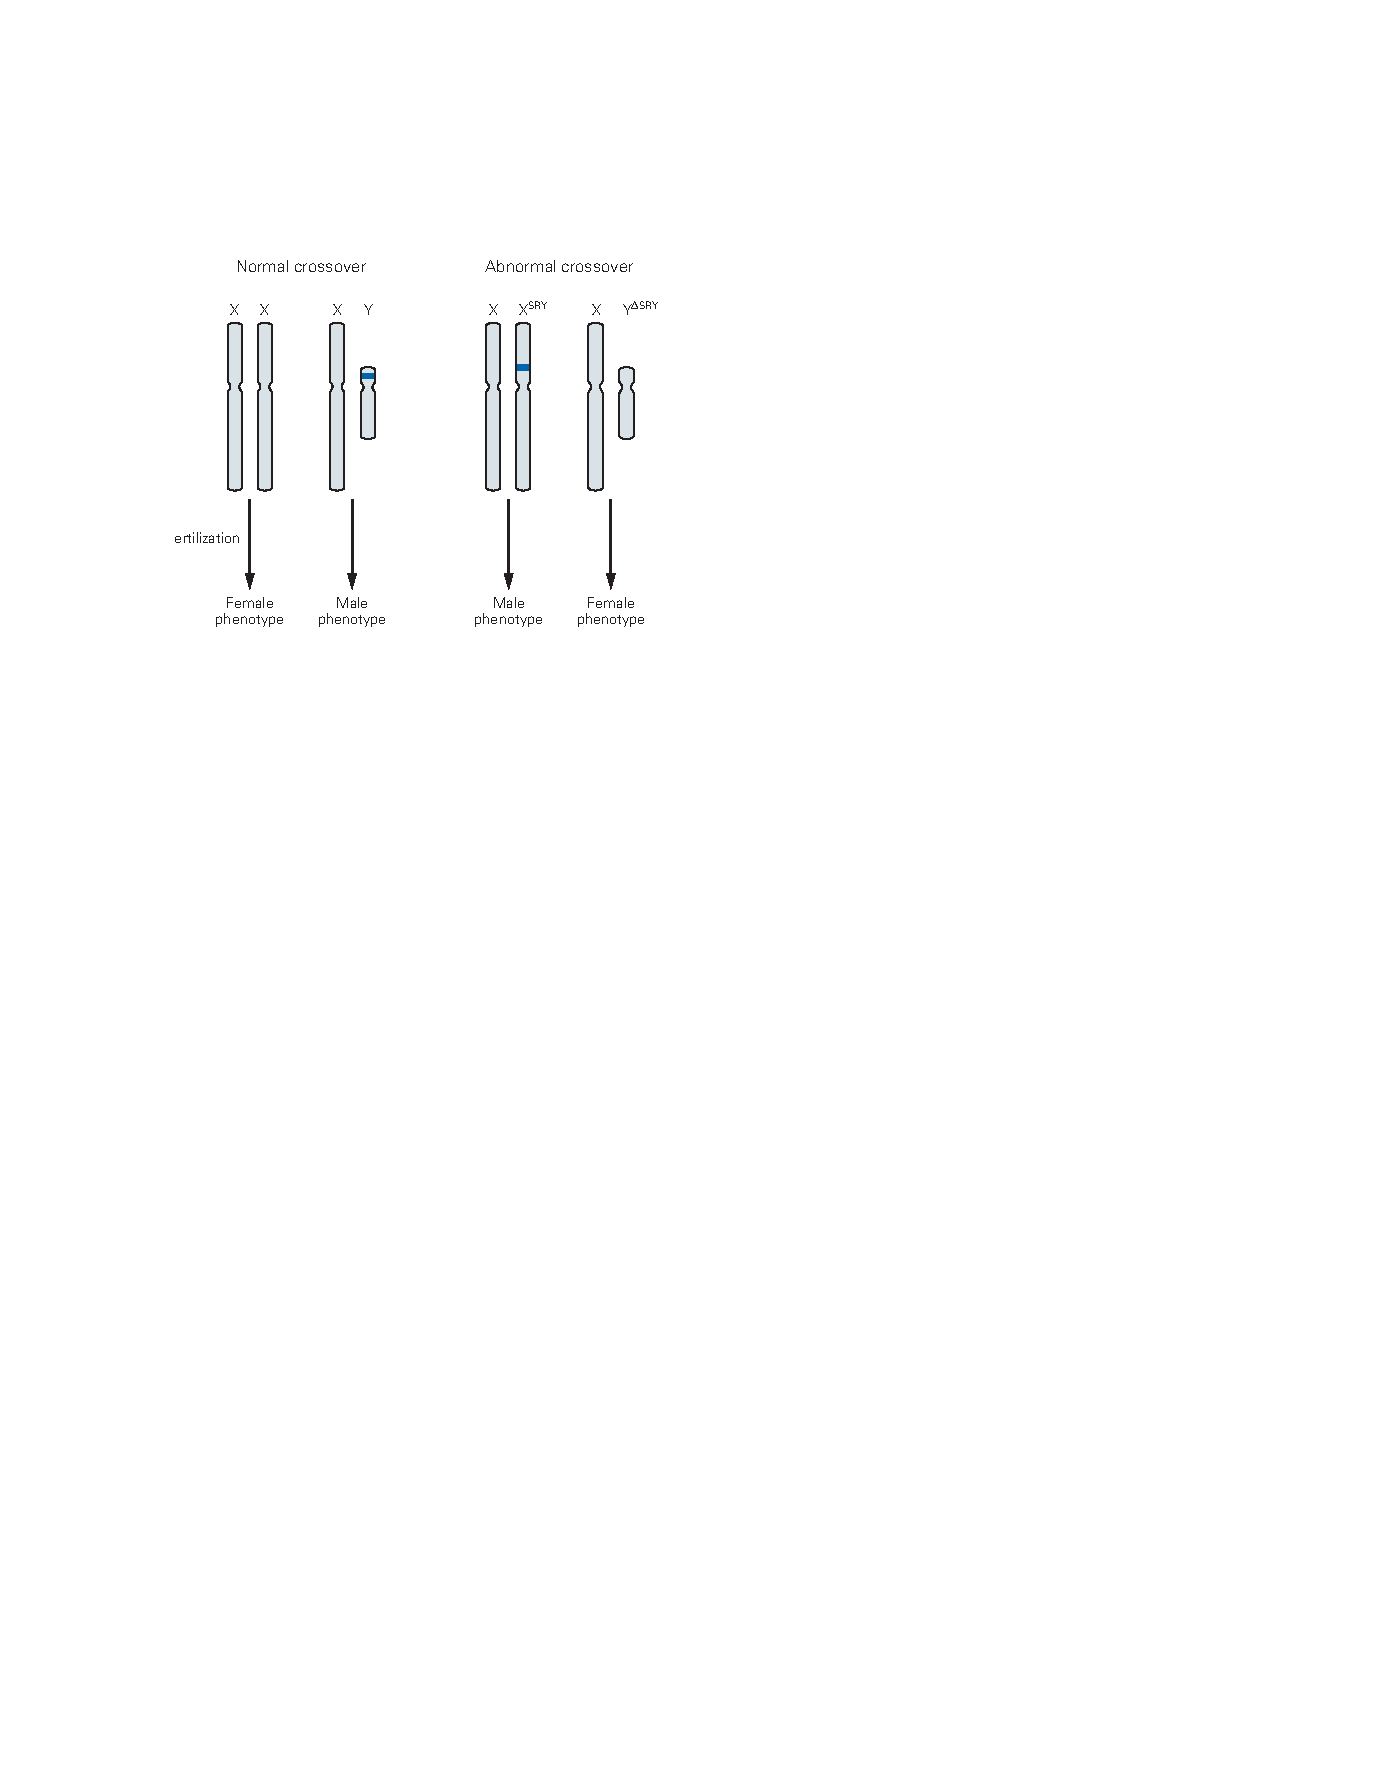
\includegraphics[width=0.61\linewidth]{chap51/fig_51_1}
	\caption{Y 染色体性别决定区基因在人类性别决定中的作用。
		Y 染色体性别决定区,性别决定位点(蓝色区域),位于 Y 染色体短臂的非同源区域。
		Y 染色体性别决定区的存在对许多哺乳动物(包括灵长类动物和大多数啮齿动物)的雄性分化具有决定性作用。
		通常携带 X 或 Y 的精子使卵母细胞受精以产生 XX 雌性或 XY 雄性,并且由此产生的表型性别与染色体性别一致。
		在极少数情况下,Y 染色体性别决定区易位至 X 染色体或常染色体(未显示)。
		在这种情况下,$ XX^{SRY} $ 后代在表型上是男性,而 $XY^{\Delta SRY}$ 后代($ \Delta $表示基因缺失)在表型上是女性\cite{wilhelm2007sex} }
	\label{fig:51_1}
\end{figure}


Y 染色体性别决定区如何指导未分化的性腺发育成睾丸?
女性差异化程序似乎是默认模式;
模式基因启动身体和性腺沿着女性特定的途径发育。
Y 染色体性别决定区基因编码一种调节基因表达的转录因子,其中一些基因会阻止默认程序的执行并启动雄性性腺分化过程。
Y 染色体性别决定区转录因子研究最深入的靶标之一是另一种转录因子 SOX9,它是睾丸分化所必需的。
因此,Y 染色体性别决定区启动了一系列诱导相互作用,最终导致男性特异性性腺发育。



\subsection{性腺合成促进性别分化的激素}

胚胎的染色体补充指导性腺的性别分化,反过来,性腺决定身体所有器官的性别特征,包括神经系统。
他们通过分泌激素来做到这一点。
性腺激素有两个主要作用。
它们的发育作用传统上被称为组织作用,因为激素对大脑和身体其他部位的早期影响导致细胞和组织分化的主要方面,通常是不可逆的。
后来,一些相同的激素会引发生理或行为反应。
这些影响通常称为激活,是可逆的。


性腺激素的组织作用的一个例子是连接性腺和外生殖器的结构分化。
在男性中,\textit{中肾管}产生输精管、精囊和附睾。
在女性中,缪勒管分化为输卵管、子宫和阴道(图~\ref{fig:51_2})。
最初,雌性(XX)和雄性(XY)胚胎都具有\textit{中肾管}和 \textit{副中肾管}。
在男性中,发育中的睾丸会分泌一种蛋白质激素、缪勒管抑制物和类固醇激素、睾酮。
缪勒管抑制物导致\textit{副中肾管}退化,睾酮诱导\textit{中肾管}分化成其成熟衍生物。
在女性中,没有 勒管抑制物允许\textit{副中肾管}分化成其成人衍生物,并且没有循环睾酮导致\textit{中肾管}吸收。
因此,Y 染色体超越女性默认程序生成男性性腺,而男性性腺又分泌激素,超越女性默认的生殖器分化程序。


\begin{figure}[htbp]
	\centering
	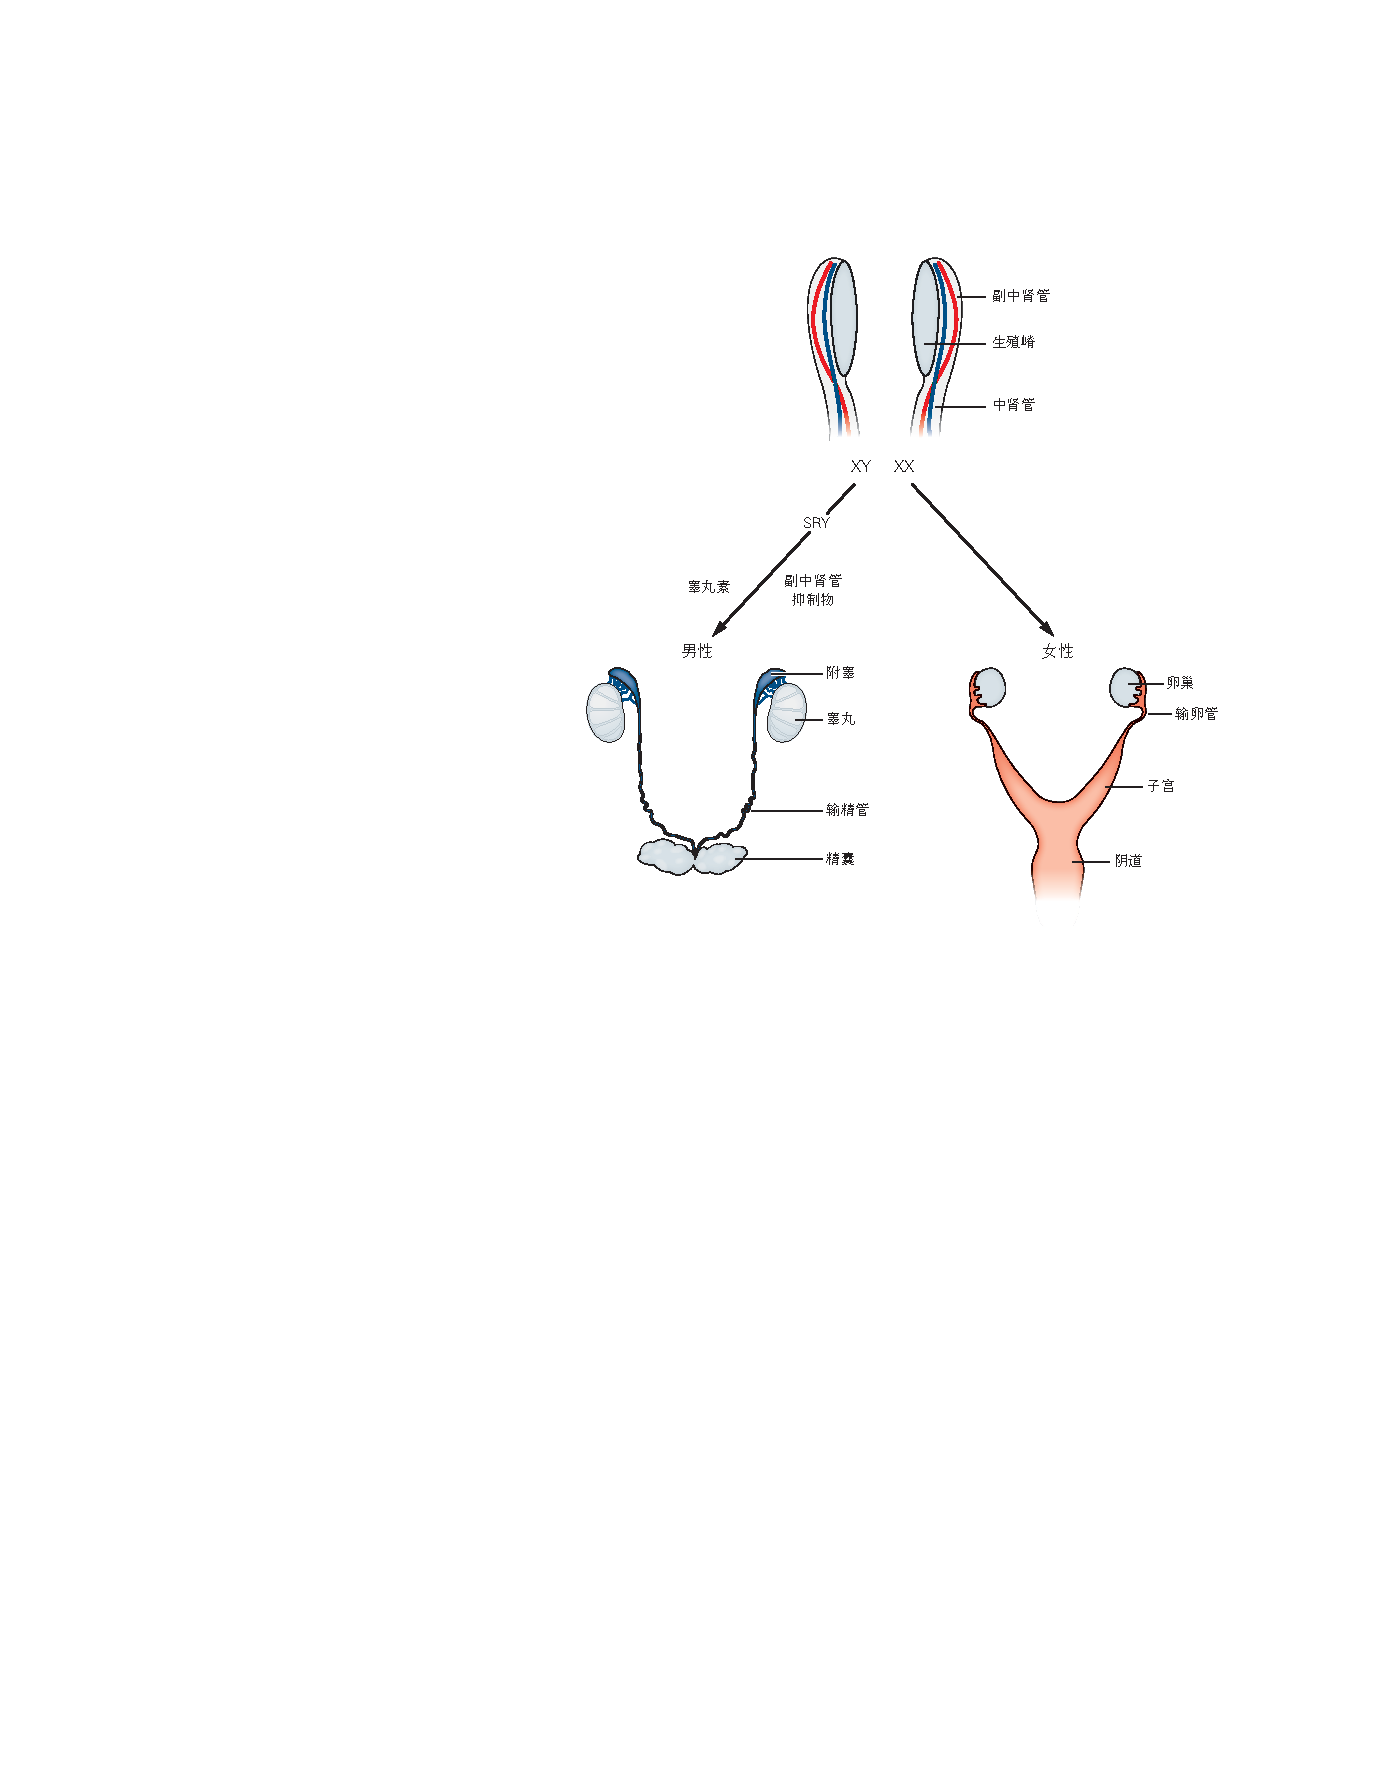
\includegraphics[width=0.77\linewidth]{chap51/fig_51_2}
	\caption{内生殖器的性别分化。
		两性的胚胎都会发育出双侧生殖脊(性腺原基),可以分化为睾丸或卵巢; 缪勒管,可分化为输卵管、子宫和阴道上段;
		\textit{中肾管}可分化为附睾、输精管和精囊。
		在 XY 胚胎中,生殖嵴中 Y 染色体性别决定区基因的表达诱导该组织分化为睾丸,\textit{中肾管}分化为男性内生殖器的其余部分,同时\textit{副中肾管}被吸收。
		在 XX 胚胎中,Y 染色体性别决定区的缺失使得生殖脊发育成卵巢,而苗勒氏管分化成女性内生殖器的其余部分;
		在没有循环睾酮的情况下,\textit{中肾管}退化\cite{wilhelm2007sex}。}
	\label{fig:51_2}
\end{figure}


缪勒管抑制物的作用主要局限于胚胎,但类固醇激素在整个生命过程中发挥作用,也就是说,它们在后期也有激活作用。 
所有类固醇激素都来源于胆固醇(图~\ref{fig:51_3})。
性类固醇可分为通常促进男性特征的雄激素和促进女性特征的雌激素加黄体酮。
睾丸主要产生雄激素睾酮,而卵巢主要产生黄体酮和雌激素 17-$ \beta $-雌二醇。
月经周期是雌激素和孕激素激活功能的一个很好的例子。


\begin{figure}[htbp]
	\centering
	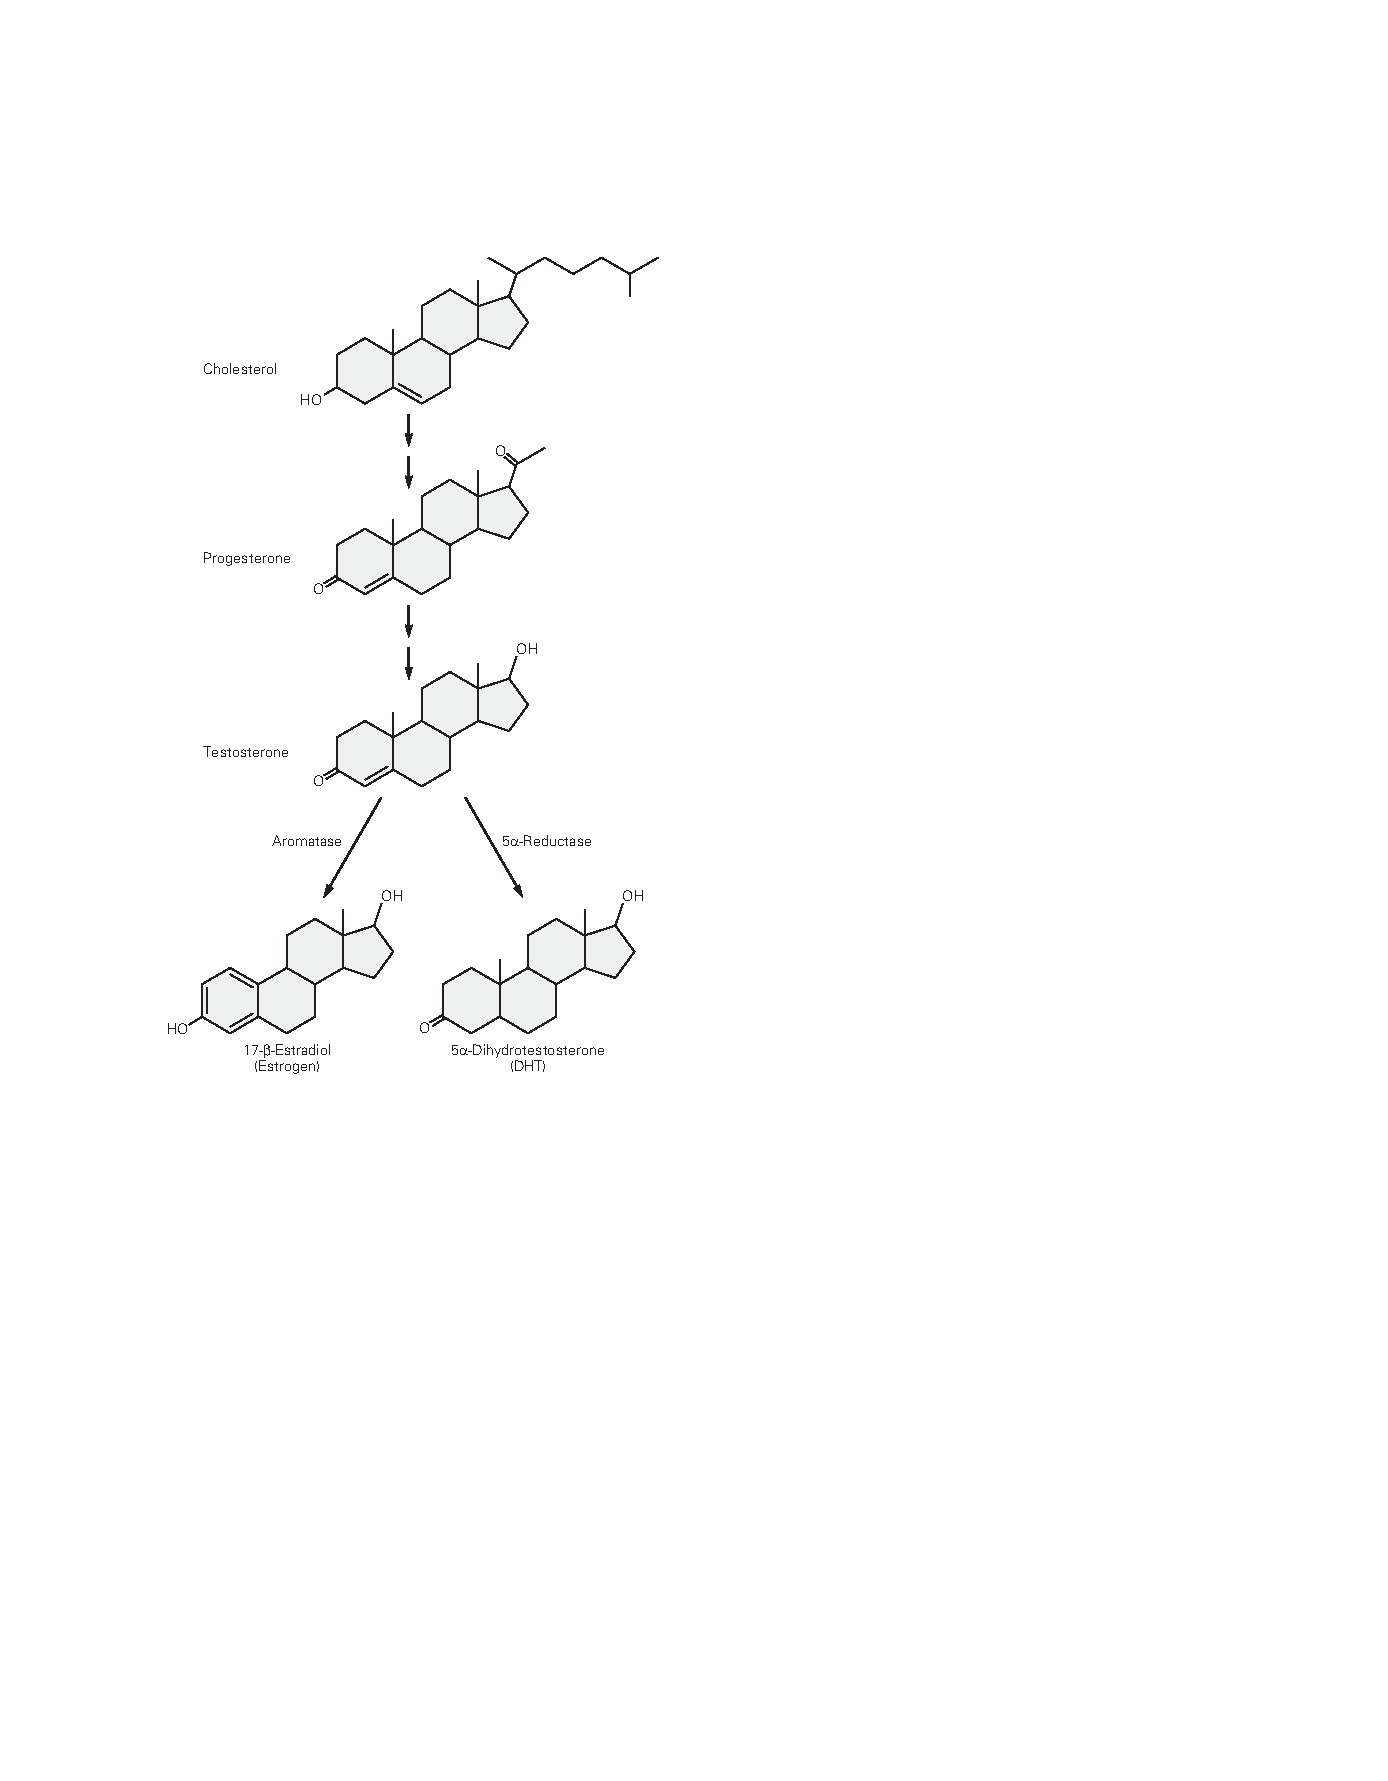
\includegraphics[width=0.64\linewidth]{chap51/fig_51_3}
	\caption{类固醇激素的生物合成。
		\textit{胆固醇}是所有类固醇激素的前体,通过一系列酶促反应转化为\textit{黄体酮}和\textit{睾酮}。
		\textit{睾酮}或相关雄激素是体内所有\textit{雌性激素}的专性前体,由一种\textit{芳香酶}催化而转化得到。
		\textit{5$\alpha$-还原酶}在靶组织中的表达将\textit{睾酮}转化为一种雄激素:\textit{5$ \alpha $二氢睾酮}。}
	\label{fig:51_3}
\end{figure}


瞥一眼类固醇激素之间的代谢关系(图~\ref{fig:51_3})就会发现一个惊喜。
女性荷尔蒙\textit{黄体酮}是男性荷尔蒙\textit{睾酮}的前体,而睾酮是女性荷尔蒙\textit{17-$ \beta $-雌二醇}的直接前体。
因此,将一种激素转化为另一种激素的酶不仅控制激素水平,而且控制激素作用的“标志”(男性或女性)。
\textit{芳香酶}是一种将睾酮转化为雌二醇的酶,它在\textit{卵巢}中含量很高,但在睾丸中含量不高。
\textit{芳香酶}的差异表达是循环睾酮和雌激素中性别二态性的原因。
\textit{芳香酶}也在大脑的不同区域表达(图~\ref{fig:51_4}A),睾酮对神经元的许多影响被认为是在其转化为雌激素后发生的。
睾酮还被\textit{5$\alpha$-还原酶}转化为另一种雄激素类固醇:\textit{5$\alpha$-二氢睾酮},存在于各种靶组织中,包括外生殖器。
在这些组织中,\textit{5$\alpha$-二氢睾酮}负责诱导次要男性特征,例如面部和体毛以及前列腺的生长。
在晚年,\textit{5$\alpha$-二氢睾酮}是男性型秃发的罪魁祸首。


\begin{figure}[htbp]
	\centering
	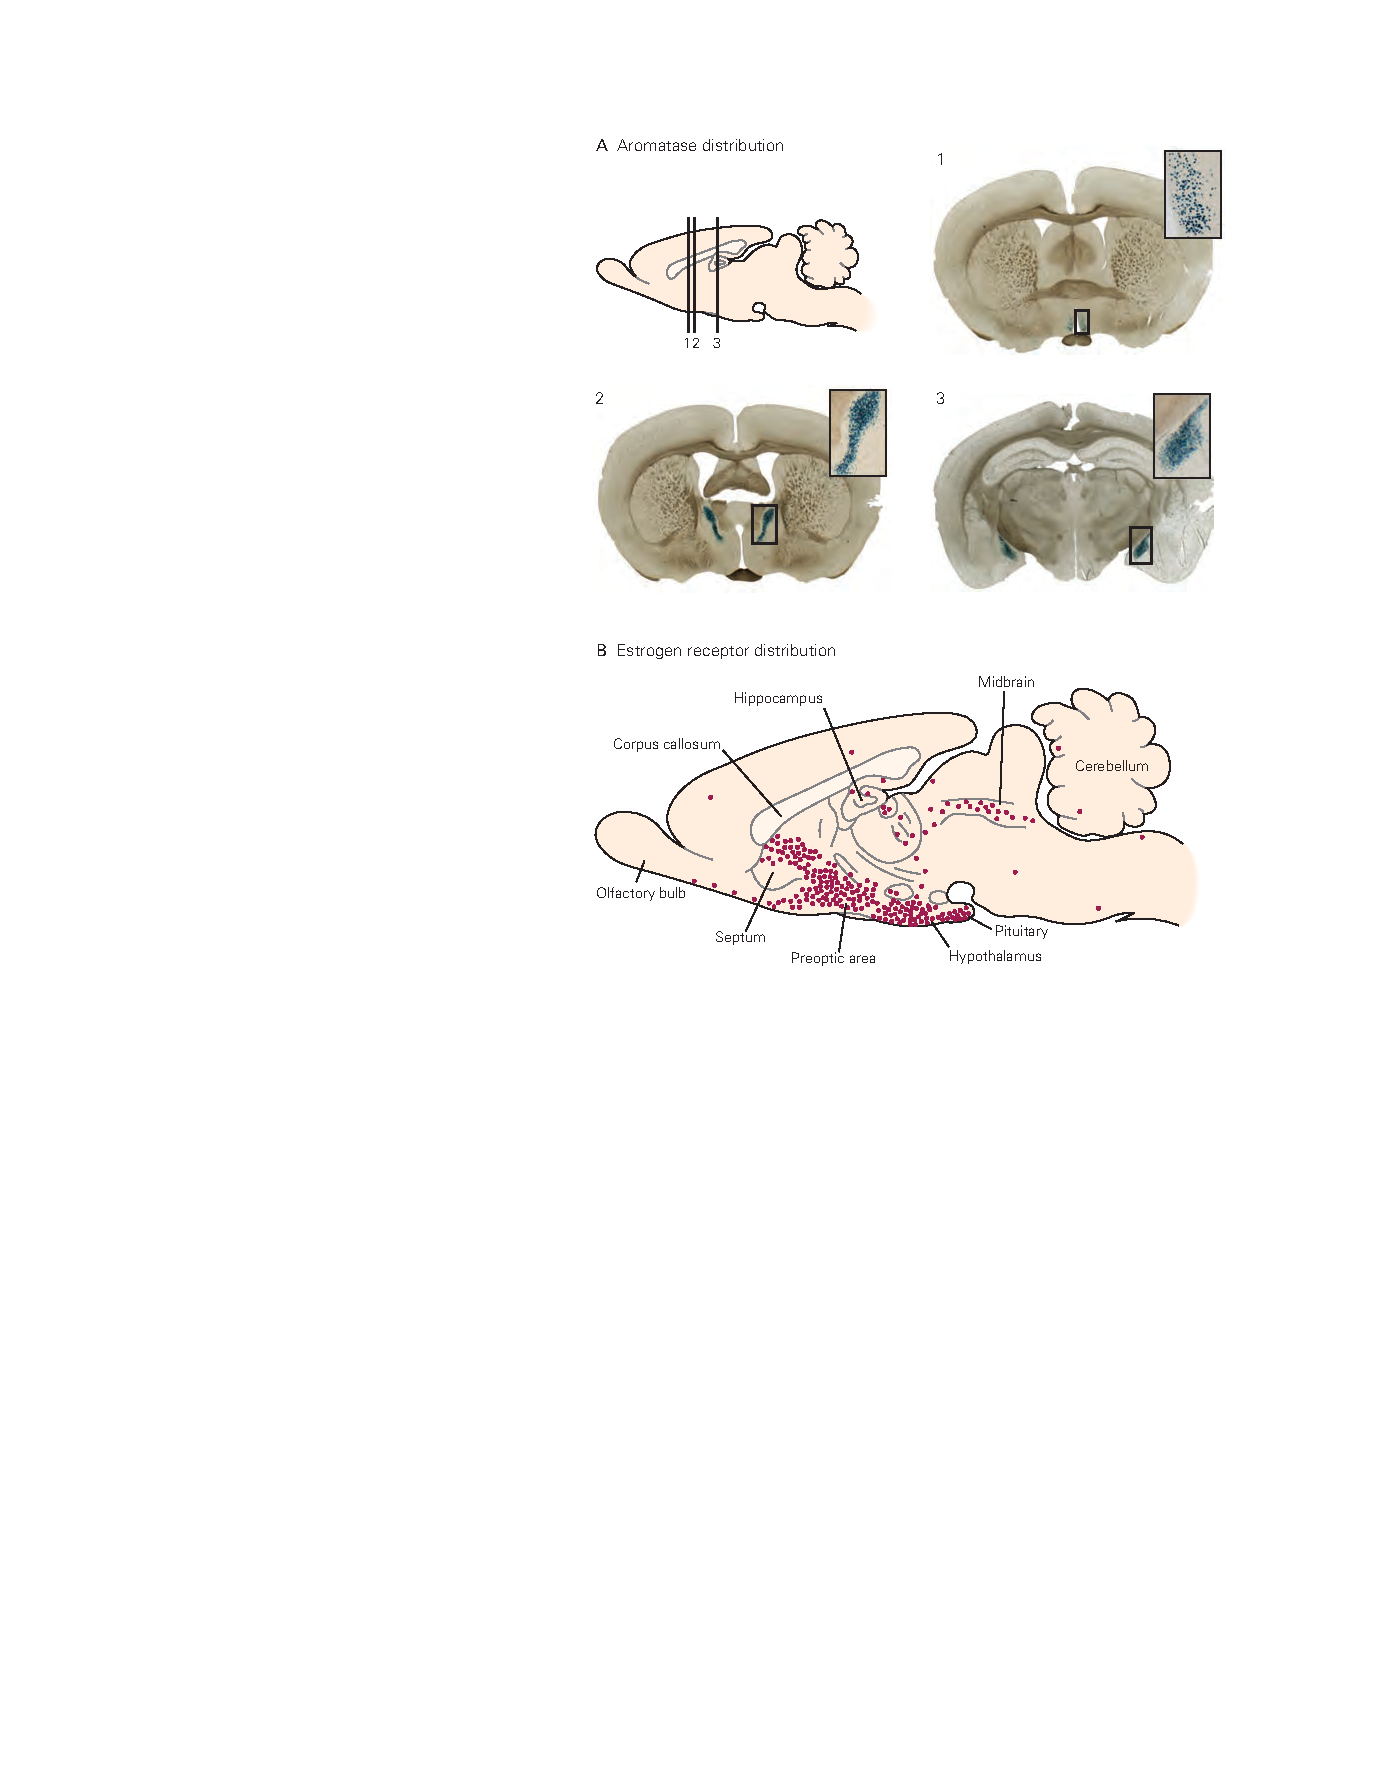
\includegraphics[width=1.0\linewidth]{chap51/fig_51_4}
	\caption{芳香酶和雌激素受体在大脑的特定区域表达。 
		\textbf{A.} \textit{芳香酶}催化\textit{睾酮}转化为雌性激素(图~\ref{fig:51_3}),并在大脑中离散的神经元群中表达。
		转基因小鼠中用报告蛋白(蓝色)标记的芳香酶表达神经元的分布显示在大脑的三个冠状平面中:
		在\textit{视前下丘脑}(1)的神经元中,在\textit{终纹床核}中(2),以及\textit{内侧杏仁核}(3)。
		这些区域包含调节性行为、攻击性和母性行为的性二态神经元\cite{wu2009estrogen}。
		\textbf{B.} 成年大鼠大脑的正中矢状切面显示雌性激素与\textit{下丘脑}各个区域的细胞结合,包括性二态性视前区。
		在\textit{隔膜}、\textit{海马体}、\textit{垂体}和\textit{中脑}中可以看到额外的雌激素结合。
		其他更侧向的区域,如杏仁核(未显示)也含有雌激素受体。}
	\label{fig:51_4}
\end{figure}



\subsection{类固醇激素生物合成障碍影响性别分化}

可以想象,编码参与类固醇激素生物合成的酶的基因突变具有深远的影响。
由此产生的表型极大地说明了类固醇激素的组织和激活作用,以及巧妙地区分两者的困难。
在这里,我们描述了三种疾病(表~\ref{tab:51_1})。


\begin{table}[htbp]
	\caption{突出雄激素在人类男性化中作用的三种临床综合症} \label{tab:51_1} \centering
	\begin{tabular}{llll}
		\toprule
		 & 完全型雄激素不敏感综合症 & 5$\alpha$-还原酶2缺乏症 & 先天性肾上腺皮质增生症\\
		\midrule
		染色体性别 & XY & XY & XY \\
		分子基础 & \makecell[l]{雄激素受体\\无功能,导致对\\循环雄激素无反应} & \makecell[l]{无功能的5$\alpha$-还原酶II\\,导致靶组织中睾酮转化\\为5$\alpha$-二氢睾酮的不足} & \makecell[l]{皮质类固醇合成\\缺陷,导致肾上腺\\循环雄激素增加} \\
		生殖腺 & 睾丸 & 睾丸 & 卵巢 \\
		中肾衍生物 & 退化的 & 现存 & 不存在 \\
		副中肾衍生物 & 不存在 & 不存在 & 现存 \\
		外生殖器 &  &  &  \\
		出生时 & 女性化 & 易变的女性化 & 可变的男性化 \\
		青春期后 & 女性化 & 男性化 & 女性化 \\
		性别认同 & 女性 & 女性或男性 & 女性或男性 \\
		性伴侣偏好 & 男性 & 女性或男性 & 女性或男性 \\
		\bottomrule
	\end{tabular}
\end{table}


第一种是\textit{先天性肾上腺皮质增生症},是肾上腺合成皮质类固醇的遗传缺陷,会导致睾酮和相关雄激素的过量产生。
这种情况是常染色体隐性遗传,每 1 万至 1 万 5 千个活产婴儿中会发生一次。
在出生时患有\textit{先天性肾上腺皮质增生症}的女孩中,过量的雄激素会导致外生殖器出现一定程度的男性化,这一过程称为男性化。
男性化清楚地反映了类固醇的组织作用。
这种情况可以在出生时被诊断出来,并通过外科手术解决。
用皮质类固醇治疗可降低睾酮水平,使这些女性能够进入青春期并变得有生育能力。


第二种遗传疾病,\textit{5$\alpha$-还原酶} II 缺乏症,也会影响性别分化。
在男性胎儿中,\textit{5$\alpha$-还原酶} II 在外生殖器的前体中高水平表达,它将循环中的睾酮转化为\textit{5$\alpha$-二氢睾酮}。
局部高浓度的\textit{5$\alpha$-二氢睾酮}使外生殖器男性化。
临床 \textit{5$\alpha$-还原酶} II 缺乏症以常染色体隐性遗传方式遗传,男性出生时外生殖器不明确(男性化不足)或明显女性化。
因此,在许多情况下,患有这种疾病的染色体男性患者(XY)在青春期之前被错误地当作女性抚养长大,此时循环睾酮的大量增加使体毛、肌肉组织以及最引人注目的外生殖器男性化。


类固醇受体在控制性分化中的关键作用在患有第三种疾病、完全\textit{雄激素不敏感综合症}的患者身上得到了很好的说明。
睾酮、雌激素和孕酮是疏水性分子,能够扩散穿过细胞膜、进入血流、进入许多器官的细胞,并与细胞内配体特异性受体结合。
这些激素的受体由不同但同源的基因编码。


单个基因编码一个受体,该受体结合雄激素睾酮和\textit{5$\alpha$-二氢睾酮}。
雄激素受体与\textit{5$\alpha$-二氢睾酮}的结合比睾丸激素的结合紧密约三倍,因此\textit{5$\alpha$-二氢睾酮}的效力更强。
还有一个\textit{黄体酮受体},而两个基因编码结合雌激素的受体(雌激素受体$\alpha$和$\beta$)。
这些类固醇激素受体存在于身体的许多组织中,包括大脑(图~\ref{fig:51_4}B)。


这些受体蛋白是结合基因组中特定位点并调节靶基因转录的转录因子。
它们包含几个标志性基序,包括激素结合域、\textit{脱氧核糖核酸}结合域和调节靶基因转录活性的域(图~\ref{fig:51_5}A)。
激素通过与受体结合激活转录活性。
在没有配体的情况下,受体与将它们隔离在细胞质中的蛋白质复合物结合。
配体结合后,受体从复合物中解离并进入细胞核,在那里它们二聚化并结合到靶基因启动子和增强子区域的特定序列元素,从而调节它们的转录(图~\ref{fig:51_5}B)。


\begin{figure}[htbp]
	\centering
	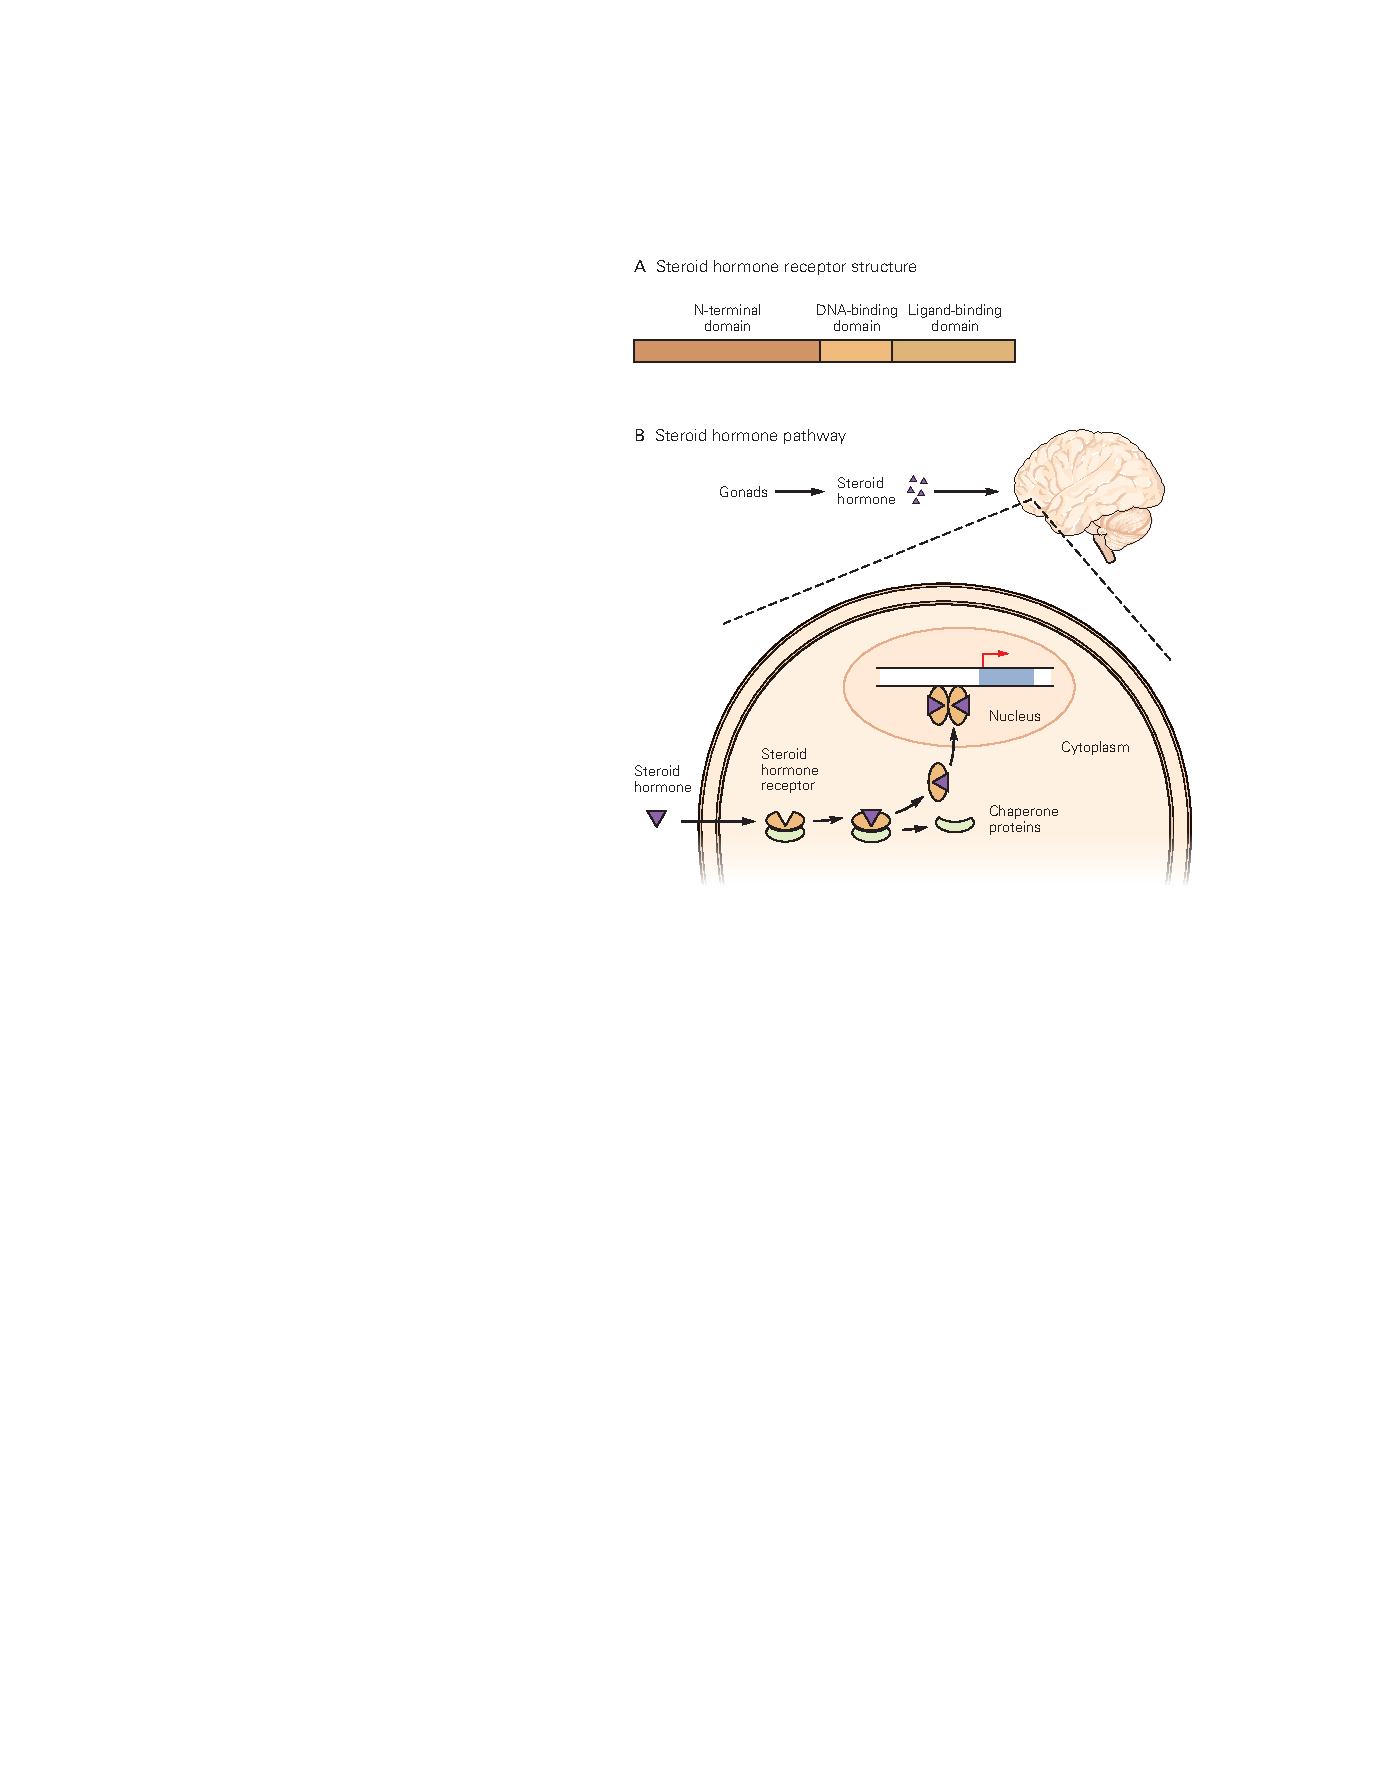
\includegraphics[width=1.0\linewidth]{chap51/fig_51_5}
	\caption{\textit{类固醇激素受体}及其作用机制。
		\textbf{A.} 类固醇激素的典型受体是配体激活的转录因子。
		这些受体有一个 \textit{N-端结构域},其中包含一个转录反式激活因子结构域;
		中央\textit{脱氧核糖核酸-结合域};
		和一个 \textit{C-端配体结合域},它可能包含一个额外的转录反式激活域。
		\textbf{B.} 性\textit{类固醇激素}是疏水性的,通过扩散穿过性腺中类固醇生成细胞的质膜进入循环。
		它们通过质膜进入远处组织(如大脑)中的靶细胞并结合它们的同源受体。
		\textit{类固醇激素受体}通常存在于与激素反应细胞的细胞质中的\textit{伴侣蛋白}的多蛋白复合物中。
		配体结合促进受体从伴侣复合物中解离并易位到细胞核中。
		在细胞核中,受体被认为作为同型二聚体与激素反应元件结合,以调节靶基因的转录\cite{wierman2007sex}。}
	\label{fig:51_5}
\end{figure}


\textit{雄激素不敏感综合症}患者的染色体为 XY,但携带 X 连锁雄激素受体的功能丧失等位基因,可消除细胞对睾酮和\textit{5$\alpha$-二氢睾酮}的反应。
由于通过 Y 染色体性别决定区进行性别决定的途径仍然有效,因此这些患者有睾丸。
然而,由于雄激素信号不足,\textit{中肾管}不发育,睾丸不能下降,外生殖器女性化。
在成年后,这些患者中的大多数选择手术切除睾丸和补充适合女性的激素。



\section{神经系统的性别分化产生两性异形行为}

性别特异性行为的发生是因为男性和女性的神经系统不同。
这些差异是由遗传因素(例如由性别决定启动的信号通路)以及环境因素(例如社会经验)共同引起的。
在许多情况下,遗传和环境输入都通过类固醇激素系统来塑造神经系统。
许多性别二态性的实例已被记录在案,包括特定结构中神经元数量和大小的差异、不同神经元群中基因表达的差异,以及连接模式和数量的差异。
在这里,我们研究了一些案例,在这些案例中,对实验动物的研究提供了见解。
在后面的部分中,我们将询问类似的机制是否是人类两性异形行为的基础。


然而,在继续之前,我们注意到性别决定的染色体机制与中枢神经系统中性别分化的细胞过程相关联的方式因物种而异。
在昆虫中,行为的性别差异与性腺的激素分泌无关,而是完全依赖于单个神经元内的性别决定途径。
这种大脑和行为的性别分化模式在果蝇中得到了很好的理解,已经证明性别决定级联启动了转录因子\textit{无效基因}的表达,它指定了雄性性行为的大部分曲目 行为(方框~\ref{box:51_1})。


\begin{figure}[htbp]
	\centering
	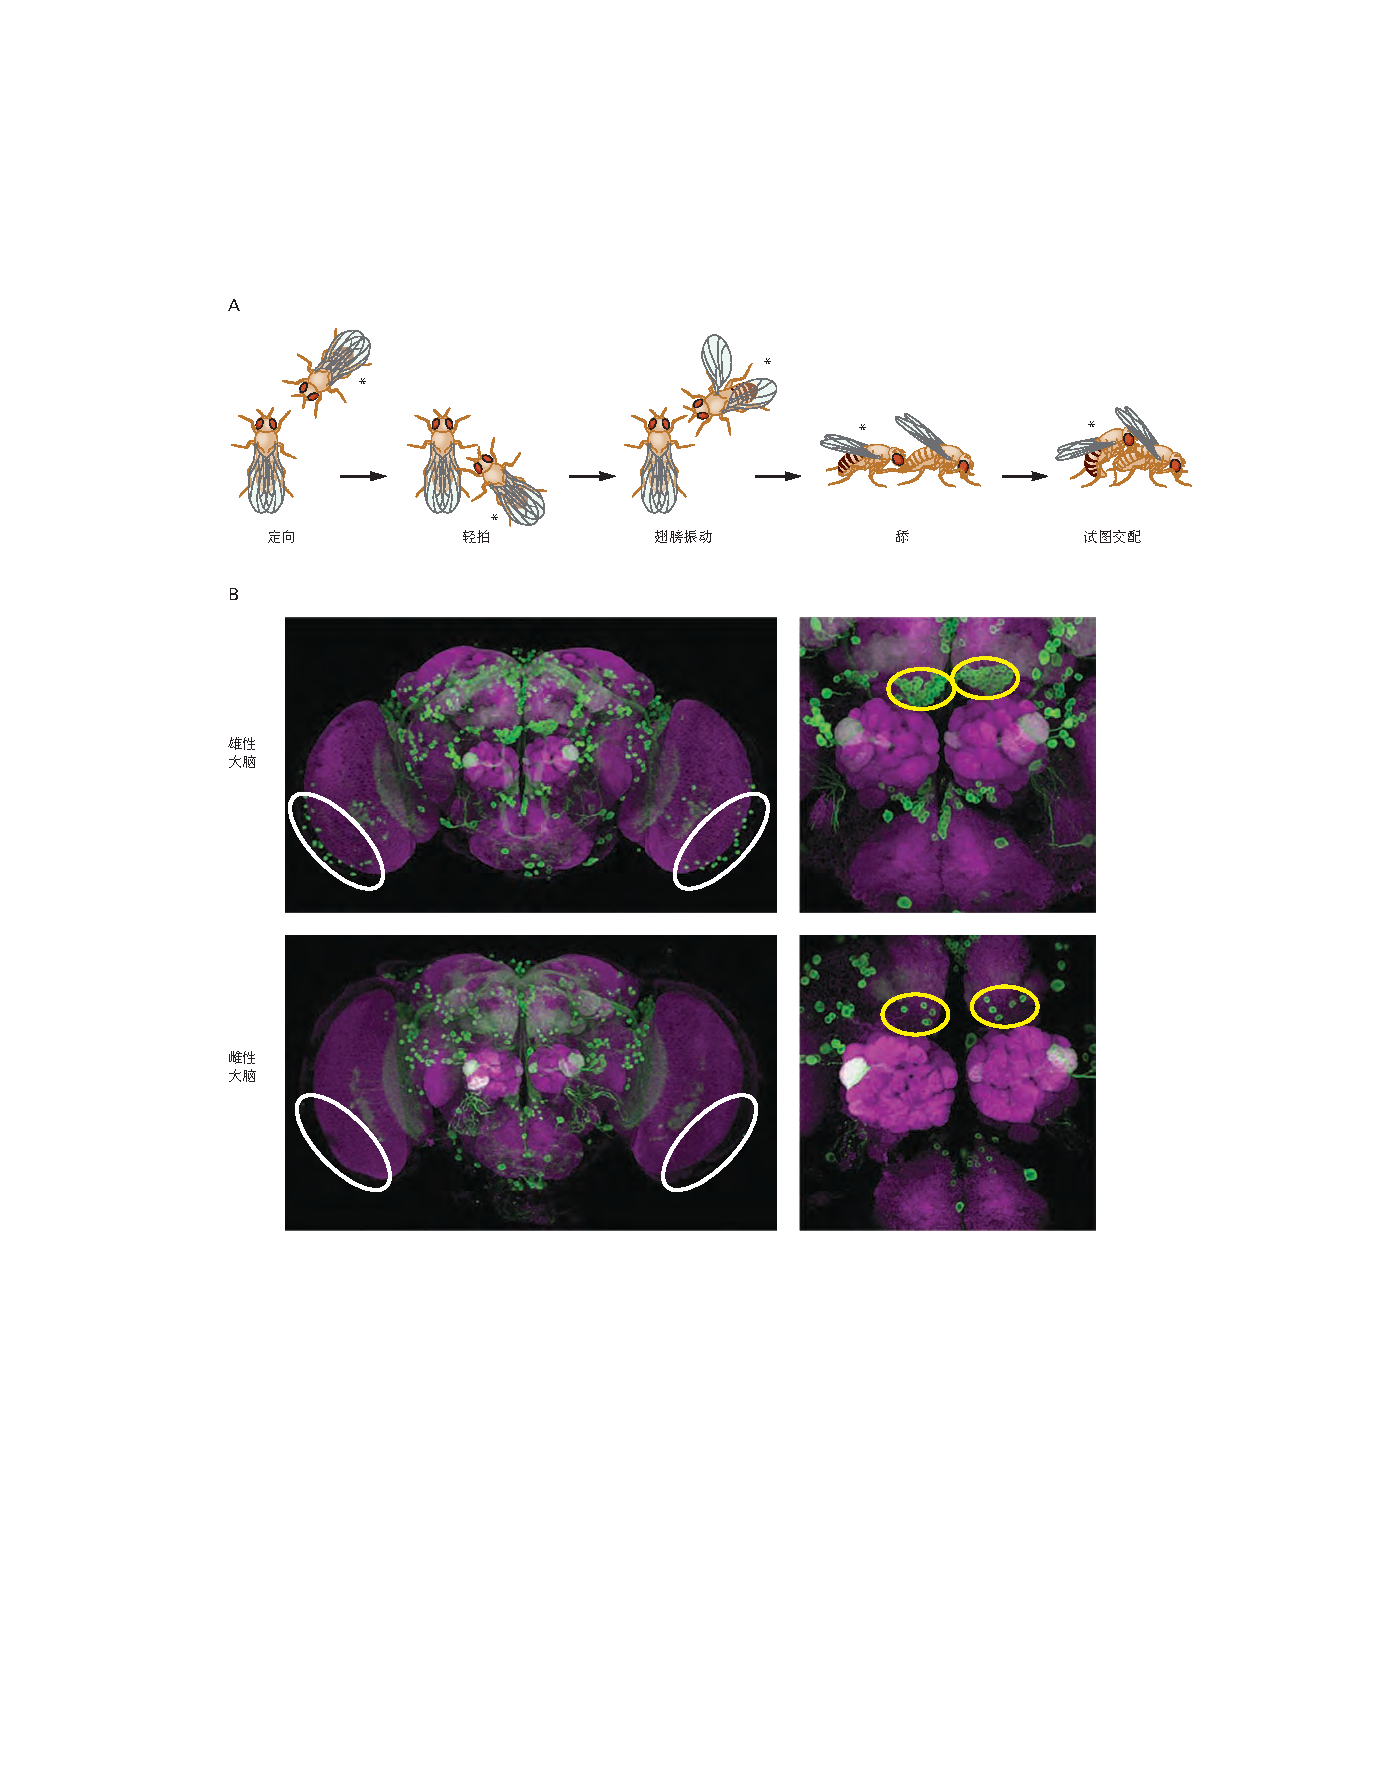
\includegraphics[width=1.0\linewidth]{chap51/fig_51_6}
	\caption{雄性果蝇求偶的控制。
		\textbf{A.} 雄性苍蝇(标有星号)参与了一系列刻板的行为惯例,最终导致试图交配。
		雄蝇朝向雌蝇,然后用前腿\textit{轻拍}她。
		其次是雄性的翅膀伸展,以及一种特定物种的\textit{翅膀振动}模式,通常被称为飞行求偶之歌。
		如果雌蝇具有性接受能力,它就会放慢速度,让雄蝇舔她的生殖器。
		然后雌性打开阴道板,让雄性开始交配。
		雄性交配仪式的所有步骤都需要表达无果(fru)基因的性别特异性剪接变体\cite{greenspan2000courtship}。
		\textbf{B.} fru基因编码雄性特异性剪接变体,这对于驱动雄性果蝇求偶仪式的大多数步骤是必要且充分的。
		在转基因果蝇中使用荧光报告蛋白(绿色)可视化\textit{无效基因}表达。
		在雄性和雌性果蝇的中枢神经系统中,表达\textit{无效基因}的神经元簇的数量相当。
		但是,\textit{无效基因}表达存在区域性别差异。
		在男性视叶(白色椭圆内的区域)中存在一簇表达\textit{无效基因}的神经元,但在女性大脑的相应区域中不存在。
		两个雄性触角叶区域(黄色椭圆内的区域)每个包含约30个神经元,而每个雌性区域只有四到五个神经元\cite{kimura2005fruitless}。}
	\label{fig:51_6}
\end{figure}


\begin{proposition}[果蝇交配行为的遗传和神经控制] \label{box:51_1}
	
	\quad \quad 在雌性果蝇的存在下,成年雄性果蝇会进行一系列基本定型的常规,通常以交配达到高潮(图~\ref{fig:51_6}A)。
	这种精心设计的男性求爱仪式是由大脑和外周感觉器官内的一系列基因转录编码的,这些基因转录使潜在的神经回路男性化。
	
	\quad \quad 苍蝇的性别决定不像脊椎动物那样依赖性腺激素。
	相反,它在整个身体中自主发生。
	换句话说,大脑和身体其他部位的性别分化与性腺性别无关。
	果蝇的雄性特异性 Y 染色体不具有性别决定基因座。
	相反,性别由X染色体数与常染色体数(X:A)的比率决定。
	1的比例决定了女性的分化,而0.5的比例决定了男性的分化。
	
	\quad \quad X:A比率启动了一系列基因转录和选择性剪接程序,导致两个基因的性别特异性剪接形式的表达,即双性(dsx)和无果(fru)。
	dsx基因编码一种转录因子,该转录因子对于神经系统和身体其他部位的性别分化至关重要,而性别特异性剪接变体则负责男性和女性的典型发育。
	
	\quad \quad fru基因编码一组由多个启动子和选择性剪接产生的推定转录因子。
	在男性中,一种特定的\textit{信使核糖核酸}(fruM)被翻译成功能蛋白。
	在雌性果蝇中,选择性剪接导致不存在此类蛋白质。
	
	\quad \quad 携带只能以女性特异性方式(fruF)剪接的转基因fru等位基因的男性基本上具有正常的dsx依赖性性别分化。
	因此,这些fruF雄性在外部类似于野生型雄性。
	然而,这些动物中FruM的丧失消除了雄性对雌性的求爱行为。
	这些数据表明,男性求偶和交配需要FruM。
	
	\quad \quad 相反,携带fruM等位基因的转基因雌性果蝇对野生型雌性表现出雄性交配行为,表明fruM足以抑制雌性性反应并促进雄性交配。
	
	\quad \quad 有趣的是,fruF雄性不追求雌性,并且像野生型雌性一样,不拒绝野生型雄性或fruM雌性的交配尝试。
	类似地,fruM雌性试图与fruM和野生型雌性交配。
	这些数据表明,fruM还可能指定性伴侣偏好,在野生型雄性的情况下,这种偏好会针对雌性。
	
	\quad \quad 在没有fruM的野生型雌性中,神经通路是连接的,因此这些苍蝇对雄性表现出性接受行为。
	当成群的雄性(或雌性)被安置在一起时,它们会激烈地相互求爱,通常会形成试图交配的长链苍蝇。
	
	\quad \quad 为了建立男性求偶仪式的基础回路,fruM似乎启动了表达它的神经元细胞自主雄性分化。
	这导致细胞数量或许多类别神经元的投射出现明显的神经解剖学二态性(图~\ref{fig:51_6}B)。
	一些表达fruM的神经元不以二态模式分布。
	在这些神经元中,fruM可能调节特定类别基因的表达,这些基因的产物驱动男性特定的生理和功能程序。
	
	\quad \quad 表达fruM的神经元是男性求偶行为所必需的吗?
	当成年男性的这些神经元中的突触传递被遗传阻断时,求偶行为的所有组成部分都被消除了。
	重要的是,这些雄性在视觉和嗅觉刺激下继续表现出正常的运动,飞行和其他行为。
	这些发现表明,fruM似乎是在一个神经回路中表达的,该神经回路对于雄性苍蝇的求偶至关重要并致力于雄性苍蝇的求偶。
	
\end{proposition}



\subsection{勃起功能由脊髓中的性二态回路控制}

许多哺乳动物(包括人类)的腰椎脊髓包含一个两性异形运动中心,即\textit{球海绵体肌脊髓核}。
\textit{球海绵体肌脊髓核}中的运动神经元支配球海绵体肌,它在男性的阴茎反射和女性的阴道运动中起着重要作用。


在成年大鼠中,雄性\textit{球海绵体肌脊髓核}比雌性\textit{球海绵体肌脊髓核}含有更多的运动神经元。
此外,雄性\textit{球海绵体肌脊髓核}运动神经元体积较大,树突状乔木较大,它们接收的突触数量相应增加。
与\textit{球海绵体肌脊髓核}运动神经元一样,男性的球海绵体肌比女性大;
它在某些哺乳动物的雌性中完全不存在。
\textit{球海绵体肌脊髓核}运动神经元还支配肛提肌,它与交配行为有关,而且男性比女性大。


这些差异是如何产生的?
最初,回路不是两性异形的。
出生时,雄性和雌性大鼠在\textit{球海绵体肌脊髓核}中具有相似数量的神经元,在球海绵体肌和提肛肌中具有相似数量的纤维。
然而,在女性中,\textit{球海绵体肌脊髓核}中的许多运动神经元以及球海绵体肌和肛提肌中的许多纤维在出生后早期死亡。
因此,这种性别二态性不是由男性特异性细胞的产生引起的,而是由女性特异性细胞死亡引起的(图~\ref{fig:51_7}A)。


\begin{figure}[htbp]
	\centering
	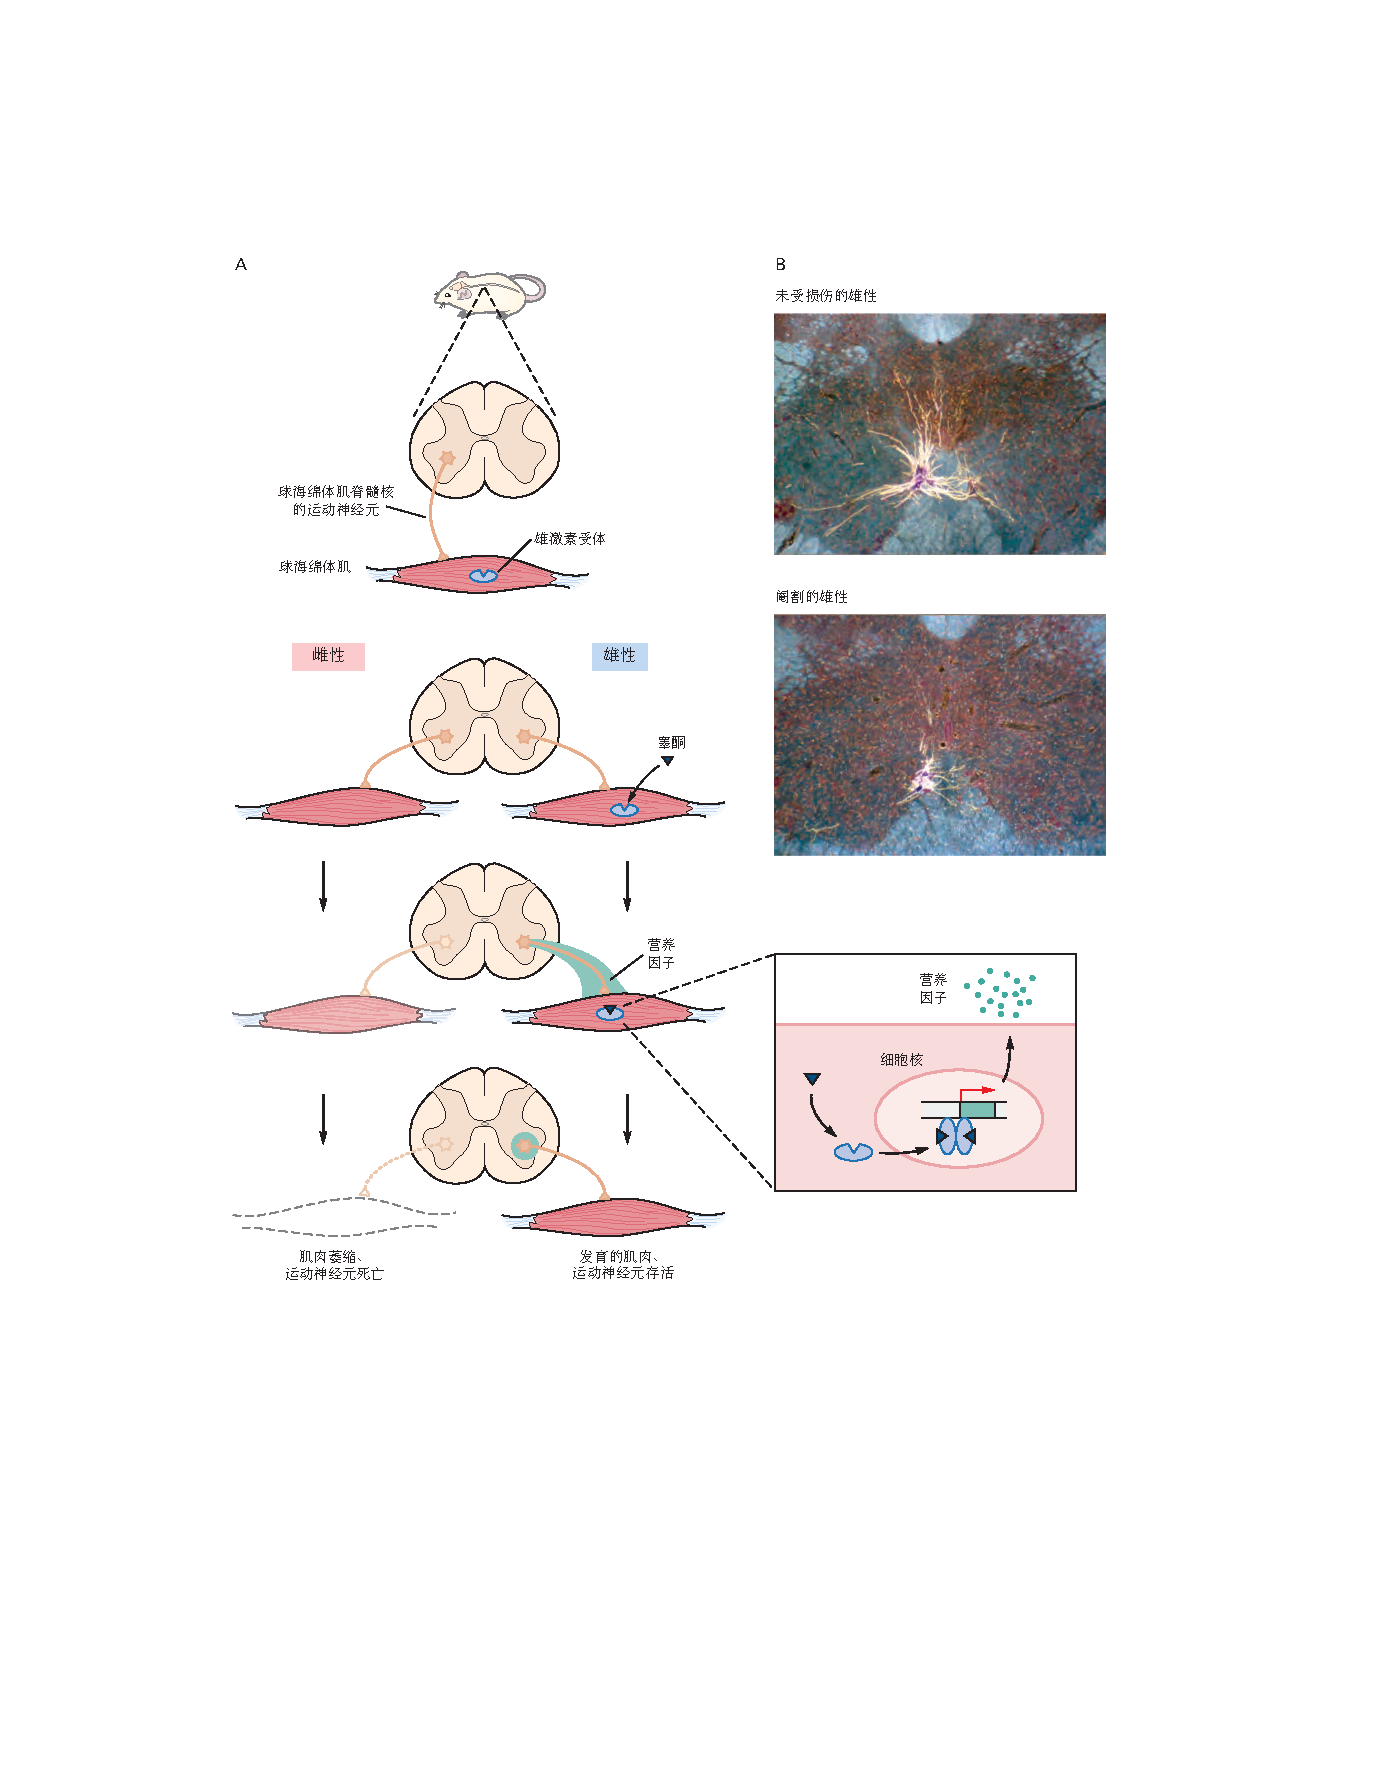
\includegraphics[width=1.0\linewidth]{chap51/fig_51_7}
	\caption{大鼠球海绵体肌脊髓核的性别二态性。
		\textbf{A.} \textit{球海绵体肌脊髓核}位于男性腰椎脊髓中,但在女性中大大减少。
		细胞核的运动神经元在出生时存在于男女两性中,但女性体内缺乏循环睾酮会导致\textit{球海绵体肌脊髓核}神经元及其目标肌肉死亡。
		据认为,男性循环中的睾酮可促进表达雄激素受体的目标肌肉的存活。
		作为对睾酮的反应,肌肉为支配\textit{球海绵体肌脊髓核}的神经元提供营养支持。
		这种源自肌肉的存活因子很可能是睫状神经营养因子或细胞因子家族的相关成员。
		因此,睾酮作用于肌肉细胞以控制\textit{球海绵体肌脊髓核}神经元的性分化\cite{morris2004sexual}。
		\textbf{B.} \textit{球海绵体肌脊髓核}神经元的树突分支受成年雄性大鼠循环睾酮的调节。
		在雄性中,树突在脊髓内广泛分枝(上图)。
		成年\textit{阉割}雄性大鼠的乔木被修剪(下图)这一事实证明这种树突状分支依赖于雄激素。
		脊髓以横截面显示,\textit{球海绵体肌脊髓核}神经元及其树突由注入目标肌肉的逆行示踪剂标记\cite{cooke2005gonadal}。}
	\label{fig:51_7}
\end{figure}


围产期注射睾酮或\textit{5$\alpha$-二氢睾酮}可以挽救雌性大鼠中大量垂死的神经元和肌肉纤维。
相反,用雄激素受体拮抗剂治疗雄性幼崽会增加垂死的神经元和肌肉纤维的数量。
所以在更深层次上,我们看到二态性是由男性特有的运动神经元和肌肉纤维的保存引起的,这些神经元和肌肉纤维在没有激素的情况下会死亡。


睾酮在哪里发挥作用来建立这种结构二态性?
它主要是运动神经元的生存因素,肌肉纤维因为失去神经支配而继发死亡吗?
或者睾丸激素是否作用于肌肉,然后提供营养因子来支持\textit{球海绵体肌脊髓核}运动神经元的存活?
这个问题已经在携带雄激素受体(tfm 等位基因)突变的大鼠中进行了检查,该突变可将配体的结合降低至正常值的 10\%。
该受体位于 X 染色体上,因此所有在其唯一且唯一的 X 染色体上携带突变基因的雄性都是女性化且不育的。
对于女性杂合子,情况更为复杂。
如前所述,每个 XX 女性的 X 染色体之一随机失活。


因此,女性杂合子是嵌合体:
一些细胞表达功能性雄激素受体等位基因,其他细胞表达突变的等位基因。
每条肌纤维都有许多细胞核,因此杂合子雌性中的大多数球海绵体肌纤维表达功能性雄激素受体。
然而,运动神经元只有一个核,因此每个神经元要么是正常的,要么是受体缺陷的。
如果神经元中需要雄激素受体,人们会认为只有表达受体的\textit{球海绵体肌脊髓核}运动神经元才能存活,而如果受体仅在肌肉中需要,人们会认为存活的运动神经元是野生型和突变体的混合体。


事实上,后一种情况发生,表明\textit{球海绵体肌脊髓核}运动神经元的存活不依赖于雄激素受体的神经元自主功能。
相反,这些神经元从雄激素依赖性球海绵体肌和提肛肌接收营养信号(图~\ref{fig:51_7}A)。
这些线索可能包括\textit{睫状神经营养因子}或相关分子,因为缺乏\textit{睫状神经营养因子}受体的突变雄性小鼠表现出\textit{球海绵体肌脊髓核}运动神经元数量减少,这是雌性的典型特征。


男性和女性\textit{球海绵体肌脊髓核}运动神经元的大小也不同。
雄激素以不同方式决定这些神经元数量和大小的差异。
对 tfm 突变体的研究表明,雄激素通过对肌肉的直接作用在出生后早期发挥组织作用。
在此关键时期雄激素水平低会导致\textit{球海绵体肌脊髓核}运动神经元数量不可逆转地减少。
后来,雄激素直接作用于\textit{球海绵体肌脊髓核}运动神经元以增加其树突状乔木的范围。
循环睾酮的流失,例如阉割后发生的睾丸激素流失,会导致树突状乔木大幅修剪;
给阉割的雄性大鼠注射补充睾酮可以恢复这种树突状分支模式(图~\ref{fig:51_7}B)。
这种影响在成年期持续存在并且是可逆的,因此可以将其视为一种激活影响。
因此,雄激素可以发挥多种作用,甚至对单一神经元类型也是如此。



\subsection{鸟类的鸣叫是由前脑中的性二态回路控制的}

几种鸣禽会学习特定物种的发声方式,用于求偶仪式和领土标记(第~\ref{chap:chap55}~章)。
一组相互连接的脑核控制着鸟鸣的学习和产生(图~\ref{fig:51_8}A)。
在一些鸣禽物种中,两性都会唱歌,而且雄性和雌性的鸣叫回路结构相似。
在其他物种中,例如斑胸草雀和金丝雀,雄性独自唱歌。
在这些物种中,雄性的几个与歌曲相关的细胞核明显大于雌性。


\begin{figure}[htbp]
	\centering
	\includegraphics[width=0.7\linewidth]{chap51/fig_51_8}
	\caption{鸟类歌曲回路中的性别二态性。
		\textbf{A.} 鸣禽有一个专门用于歌曲制作和学习的神经回路,其中不同的组件有助于学习或创作。
		这些成分中的许多在只有一种性别的鸣禽中是两性异形的。
		例如,在斑胸草雀中,只有雄性会唱歌,而雄性\textit{高级发声中枢}、\textit{古纹状体强健核}、\textit{新纹状体前部大细胞核外侧部}和 X 区体积较大, 比女性的可比区域包含更多的神经元\cite{brainard2002songbirds}。
		\textbf{B.} 在雄性中,\textit{高级发声中枢}神经元的轴突终止于\textit{古纹状体强健核}细胞核中的神经元,而在女性中,轴突终止于细胞核周围的区域。
		这些区域的细胞数量和连通性的性别二态性受雌激素调节\cite{morris2004sexual}。
		\textbf{C.} \textit{古纹状体强健核}中\textit{高级发声中枢}神经元轴突的终止模式在孵化后的不同年龄的雄性和雌性中有所不同\cite{konishi1985neuronal}。 }
	\label{fig:51_8}
\end{figure}


已经在斑胸草雀中详细研究了歌曲回路中两性异态的发展。
成年雄性斑胸草雀健壮的\textit{古纹状体强健核}包含的神经元数量是雌性相同核的五倍。
此外,对\textit{古纹状体强健核}的传入投射表现出显著的性别二态性,仅在男性中,\textit{古纹状体强健核}才接收来自\textit{高级发声中枢}的输入(图~\ref{fig:51_8}B)。
\textit{古纹状体强健核}的细胞数量和连通性的这些性别差异直到孵化后才明显,此时在雌性中大量\textit{古纹状体强健核}神经元死亡,而在雄性中\textit{高级发声中枢}神经元的轴突进入\textit{古纹状体强健核}细胞核。


这些两性异形的解剖学特征受类固醇激素的调节。
当雌性在孵化后被提供雌激素(或可芳香化的雄激素,如睾酮)时,\textit{古纹状体强健核}中的神经元数量和细胞核中的终止模式与雄性相似。
然而,早期对年轻雌性进行激素给药不足以使歌曲核雄性化至与成年雄性相当的大小,也不足以诱导雌性唱歌。
为了实现这些功能,孵化后接受睾酮或雌二醇的雌性鸟类成年后也必须接受睾酮或二氢睾酮(但不包括雌激素)。
因此,类固醇在该系统中也起着组织和激活的作用。



\subsection{哺乳动物的交配行为受下丘脑中的性二态神经回路控制}

在许多哺乳动物物种中,下丘脑的视前区和相互连接的区域,即\textit{终纹床核},在两性异形交配行为中起着重要作用(第~\ref{chap:chap41}~章;图~\ref{fig:51_4})。
在雄性啮齿动物和猴子中,这些区域在交配行为中被激活;
切除视前区或\textit{终纹床核}的手术损伤会导致雄性啮齿动物的雄性性行为缺陷,并且在视前损伤的情况下,会抑制雄性的雌性性接受能力。


视前下丘脑和\textit{终纹床核}都是性二态的,与女性相比,男性的神经元更多。
\textit{视前区性二态核团}在男性中也包含明显更多的神经元。
男性特有的围产期睾酮激增促进了\textit{视前区性二态核团}和\textit{终纹床核}中神经元的存活,而在女性中,这些相同的细胞在出生后早期逐渐死亡。
这种发展类似于啮齿动物脊髓和鸣禽大脑的性二态细胞核,表明雄激素控制是神经元数量性别差异产生的常见机制。


奇怪的是,大脑睾酮促进神经元存活的能力很可能是通过芳构化为雌激素并随后激活雌激素受体来发挥作用的(见图~\ref{fig:51_3}~和~\ref{fig:51_4})。
那么,新生儿女性大脑如何免受循环雌激素的影响呢?
在新生女性中,循环中的雌激素很少,而且少量的雌激素很容易通过与血清蛋白甲胎蛋白结合而被隔离。
这解释了为什么缺乏甲胎蛋白的雌性小鼠表现出雄性典型行为并降低了雌性典型性接受能力。
那么,在这种情况下,结构性二态性不是由雄激素和雌激素的不同作用引起的,而是由于靶组织可用激素水平的性别差异引起的。



\section{环境线索调节两性异形行为}

特定性别的行为通常是响应环境中的感官线索而发起的。
有许多这样的线索,不同的物种使用不同的感觉方式来引发相似的反应。
求偶仪式可以由特定物种的发声、视觉信号、气味触发,甚至在弱电鱼的情况下,可以由放电触发。
最近的遗传和分子研究使人们对感官体验如何控制啮齿动物的某些行为有了重要的了解。
在这里,我们讨论两个例子:信息素对伴侣选择的调节和婴儿期经验对母性行为的调节。



\subsection{信息素控制小鼠的伴侣选择}
许多动物依靠嗅觉四处走动、获取食物和躲避捕食者。
它们还依赖信息素:一种动物产生的化学物质来影响该物种另一成员的行为。
在啮齿动物中,信息素可以引发许多性二态行为,包括择偶和攻击行为。


信息素由脊椎动物鼻子中两个不同感觉组织中的神经元检测:\textit{主嗅上皮}和\textit{犁鼻器}(图~\ref{fig:51_9}A)。
人们认为\textit{主嗅上皮}中的感觉神经元检测挥发性气味,而\textit{犁鼻器}中的感觉神经元检测非挥发性化学感觉线索。
去除嗅球(\textit{主嗅上皮}和\textit{犁鼻器}中神经元的唯一突触目标)会消除小鼠和其他啮齿动物的交配和攻击行为。
这些和其他研究表明嗅觉刺激在开始交配和战斗中起着重要作用。


\begin{figure}[htbp]
	\centering
	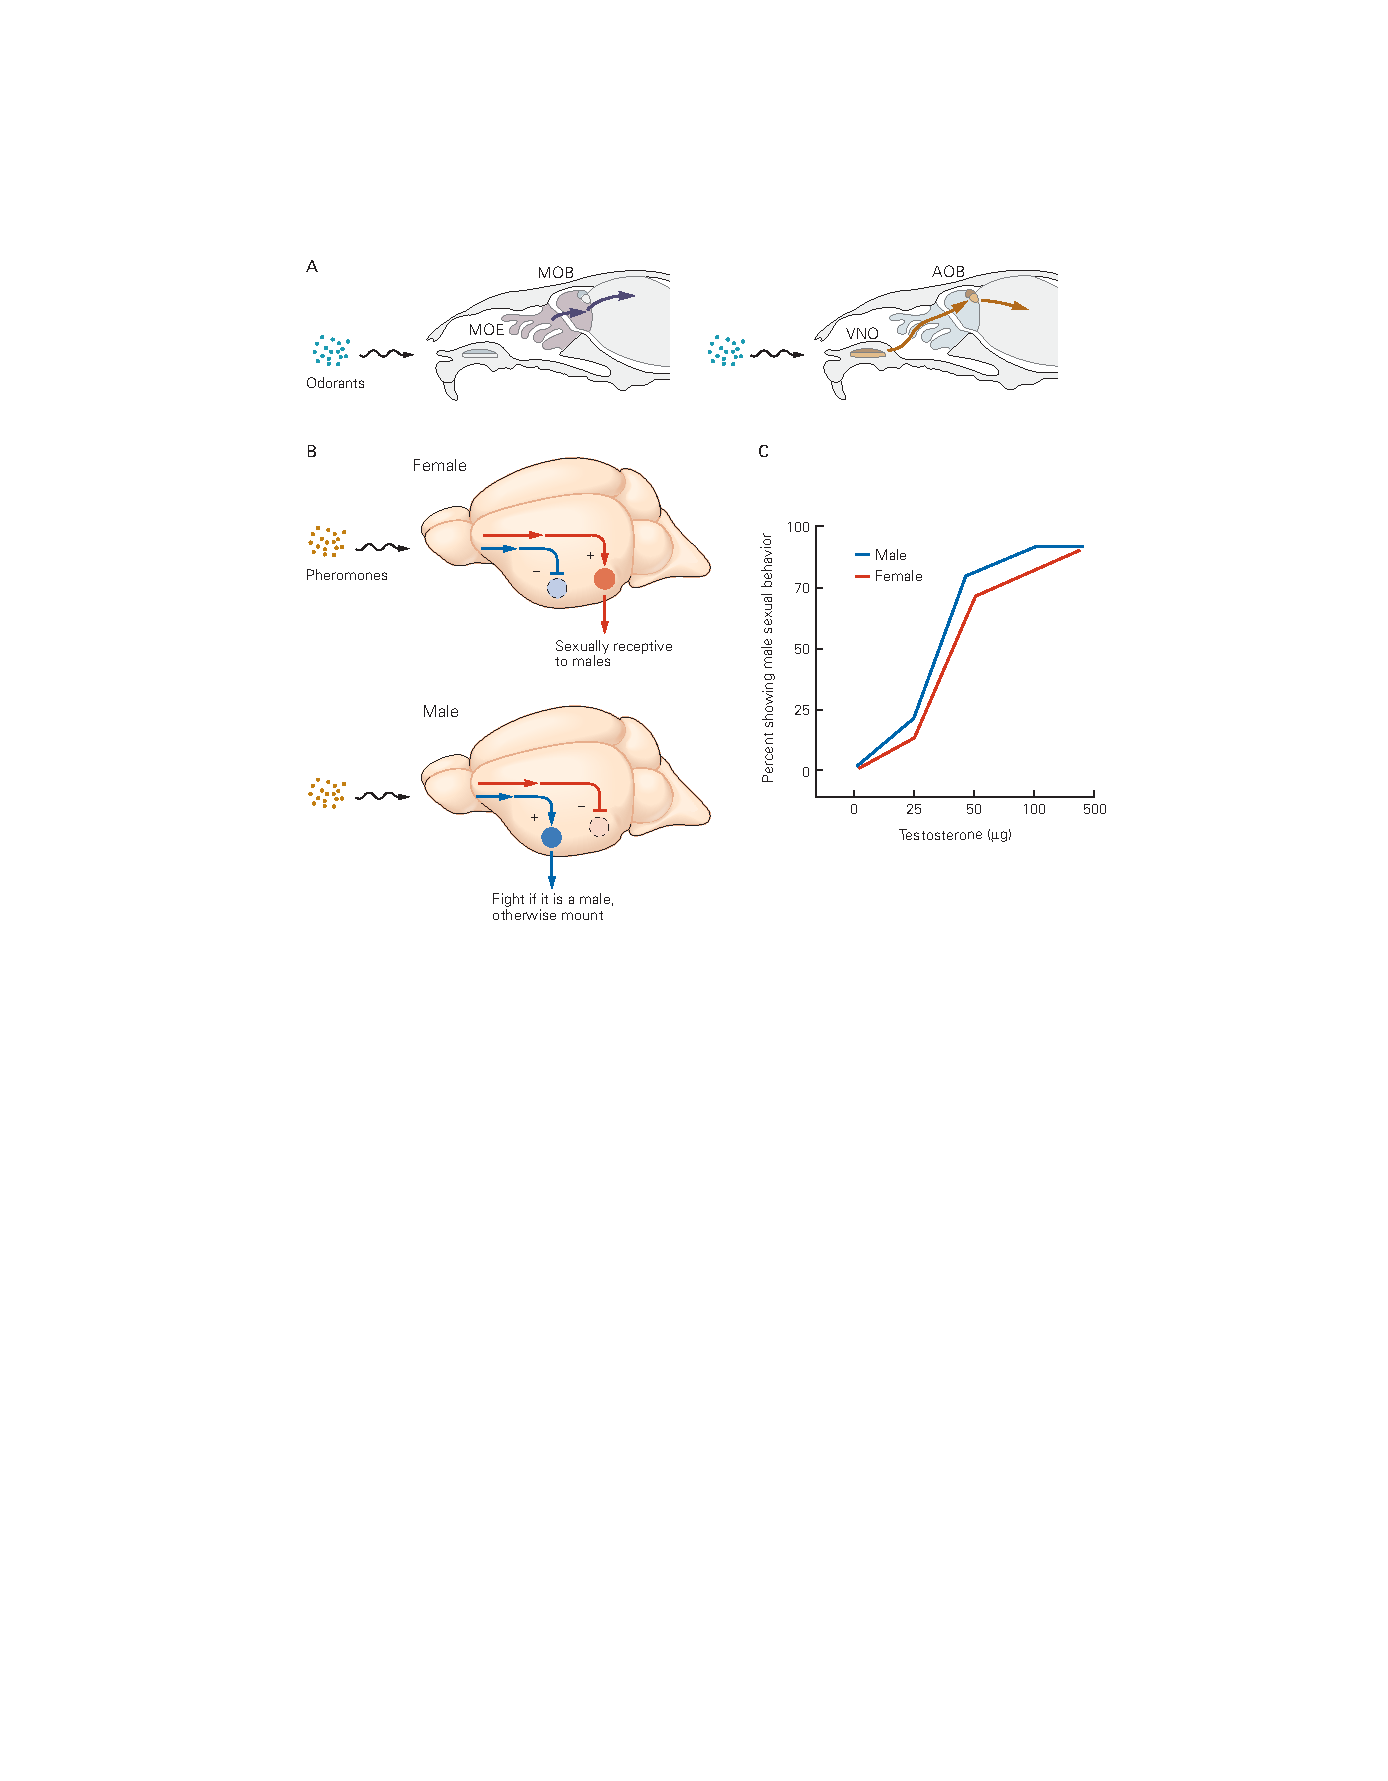
\includegraphics[width=0.95\linewidth]{chap51/fig_51_9}
	\caption{小鼠性二态行为的信息素和荷尔蒙控制。
		\textit{主嗅上皮} \textit{主嗅上皮}中的感觉神经元检测到气味,它投射到\textit{主嗅球},\textit{犁鼻器}中的神经元投射到\textit{副嗅球}。
		\textit{主嗅上皮}和\textit{犁鼻器}通路的许多中心连接在解剖学上是分离的\cite{dulac2006genetic}。
		\textbf{B.} 雌性小鼠拥有可以激活雄性(蓝色)或雌性(红色)交配行为的神经回路。
		在野生型雌性中,信息素激活雌性交配行为并抑制雄性交配。
		相比之下,在雄性中,信息素会激活一个回路,该回路将启动与雄性的战斗并与雌性交配\cite{kimchi2007functional}。
		\textbf{C.} 睾酮激活雄性和雌性小鼠的雄性性行为。
		这些数据来自一项研究,其中雄性和雌性小鼠的性腺在成年期被手术切除。
		手术后,没有一只动物表现出与野生型雌性的雄性性行为。
		施用睾酮后,被阉割的雄性恢复了交配行为,而雌性则表现出雄性性行为。
		这种作用是剂量依赖性的;
		在最高剂量下,雄性和雌性小鼠对野生型雌性表现出相当水平的雄性交配行为\cite{edwards1971early}。 }
	\label{fig:51_9}
\end{figure}


通过基因工程破坏\textit{主嗅上皮}或\textit{犁鼻器}中的信息素反应表明,这些感觉组织在小鼠的交配行为中具有惊人的复杂作用。
功能性\textit{主嗅上皮}对于触发男性性行为至关重要,而完整的\textit{犁鼻器}是性别歧视和指导男性与女性交配所必需的。


这些实验的关键是\textit{主嗅上皮}和\textit{犁鼻器}中的嗅觉神经元使用不同的信号转导级联将嗅觉输入转化为电反应。
阳离子通道 Trpc2 似乎对\textit{犁鼻器}神经元中信息素诱发的信号传导至关重要;
它不在使用不同信号转导装置的\textit{主嗅上皮}神经元中表达。
因此,缺少基因 trpc2 的小鼠具有无功能的\textit{犁鼻器}和完整的\textit{主嗅上皮}。
针对异性动物的交配行为在 trpc2 突变雄性和雌性中似乎没有改变。


然而,男性和女性 trpc2 突变体通常表现出与任何性别成员的男性性行为。
例如,trpc2 突变体雌性与雌性交配的方式似乎与野生型雄性没有区别,当然雌性不能射精。
这些和其他调查结果表明,\textit{犁鼻器}被用来歧视性伴侣。
当\textit{犁鼻器}失活时,动物无法再区分雄性和雌性,因此突变体对两性成员都表现出雄性性行为。
同样,用睾酮治疗的成年野生型雌性也表现出雄性对雌性的性行为(图~\ref{fig:51_9}C)。


这些研究的一个含义是雌性小鼠拥有雄性性行为的神经回路(图~\ref{fig:51_9}B)。
这种神经回路的激活在野生型雌性中受到来自\textit{犁鼻器}的感觉输入和缺乏睾酮的抑制。
去除\textit{犁鼻器}或施用睾酮可激活女性的男性性行为。
在许多物种的雌性身上都观察到了雄性模式的交配行为,这表明在老鼠身上的发现可能具有普遍意义。
因此,男性性行为的神经通路似乎存在于两性中。
同样,雄性大鼠在下丘脑损伤后的典型雌性行为表明,雌性性行为的神经通路也存在于雄性大脑中。
在这种情况下,正是这些回路的不同调节构成了男性和女性性行为的性二态表达的基础。



\subsection{早期经验改变了后来的母性行为}

下丘脑的视前区和\textit{终纹床核}对于女性的另一组性二态行为也很重要。
护理啮齿动物是好母亲,为它们的幼崽筑巢,蹲伏在幼崽身上为它们取暖,并在幼崽碰巧爬走时将它们送回巢穴。
视前区的手术损伤或实验性刺激分别消除或激活了这些母性行为。


对这些行为的研究揭示了雌性个体之间的差异,以及这些差异如何对后代的行为产生终生影响。
雌性实验室大鼠表现出独特、稳定的母性护理形式:一些经常\textit{舔舐和梳理}幼鼠(高\textit{舔舐和梳理}母亲),而另一些则不那么频繁地舔和梳理(低\textit{舔舐和梳理}母亲)。
与低\textit{舔舐和梳理}母亲的雌性后代相比,高\textit{舔舐和梳理}母亲的雌性后代在自己成为母亲时表现出高\textit{舔舐和梳理}活性(图~\ref{fig:51_10})。
此外,与低\textit{舔舐和梳理}母亲的幼崽相比,高\textit{舔舐和梳理}母亲的幼崽在压力条件下表现出更少的焦虑样行为。


\begin{figure}[htbp]
	\centering
	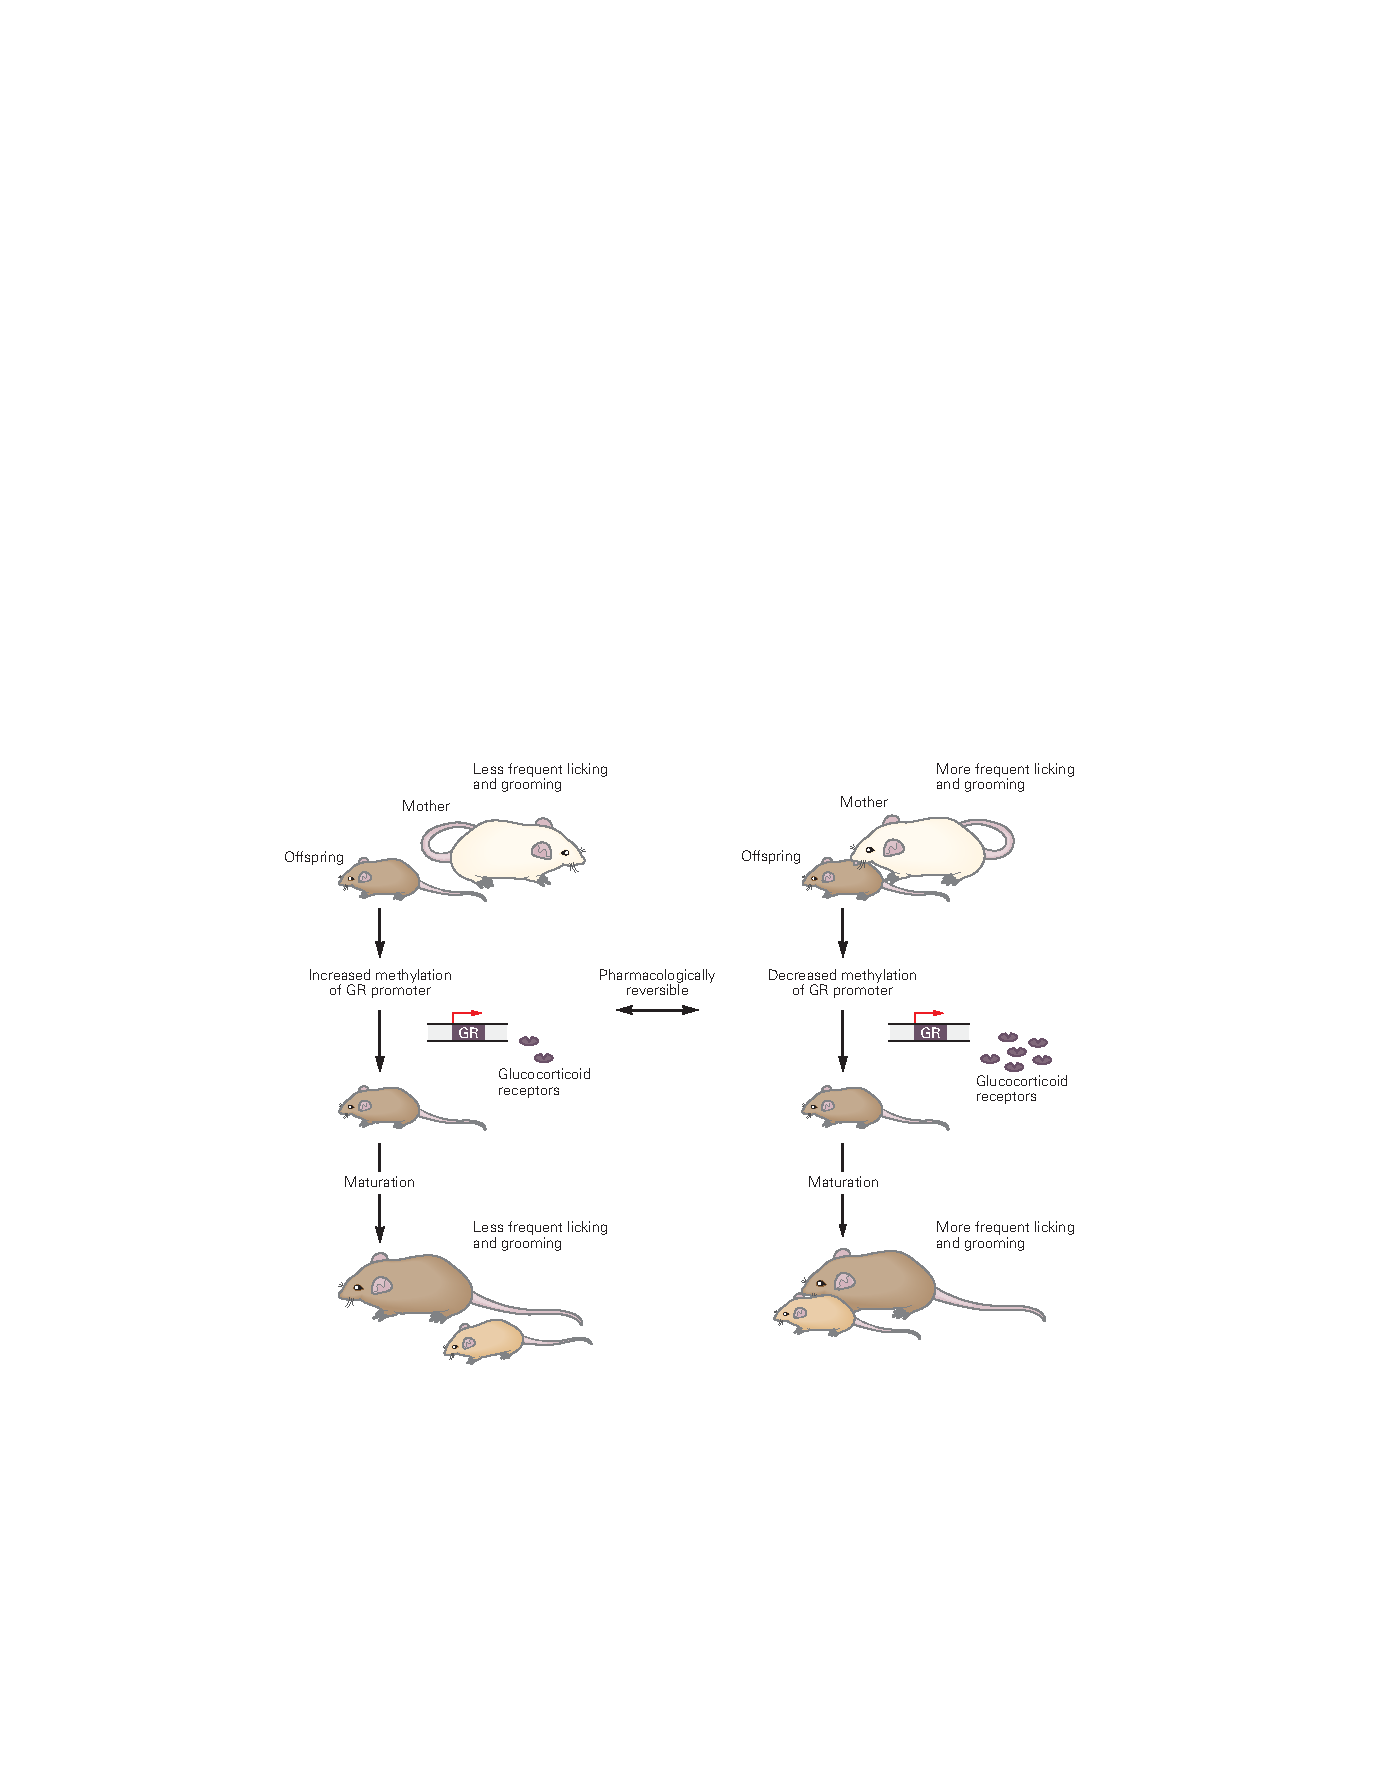
\includegraphics[width=0.97\linewidth]{chap51/fig_51_10}
	\caption{大鼠母性行为的表观遗传调控。
		在一种常见的实验室大鼠品系中,不同的母亲以低频或高频舔舐和梳理幼崽,导致\textit{糖皮质激素受体}启动子发生明显的表观遗传修饰。
		频繁舔毛和梳理毛发的母亲会在\textit{糖皮质激素受体}启动子处培育出低水平\textit{脱氧核糖核酸}甲基化的后代,从而导致海马体中更高水平的\textit{糖皮质激素受体}表达。
		由这些母亲抚养长大的雌性对自己的幼崽表现出更高频率的舔舐和梳理行为。
		以低频率舔毛和梳理毛发的母亲在\textit{糖皮质激素受体}启动子处培育出具有高\textit{脱氧核糖核酸}甲基化水平和海马\textit{糖皮质激素受体}表达水平较低的后代。
		由这些母亲哺育的雌性随后表现出类似的低水平舔舐和梳理它们的幼崽。
		\textit{糖皮质激素受体}启动子表观遗传修饰的药理学逆转导致\textit{糖皮质激素受体}表达和母性行为的相应变化\cite{sapolsky2004mothering}。}
	\label{fig:51_10}
\end{figure}


这些结果表明,舔舐和梳理行为的水平以及应激反应是由基因决定的。
然而,\textit{迈克尔$\cdot$米尼}及其同事的研究提供了另一种解释。
当雌性幼鼠在出生时从它们的母亲转移到养母时,它们成年后的母性行为和压力反应类似于它们的养母,而不是它们的亲生母亲。
因此,婴儿期的经历可以导致终生的行为模式。
由于这些模式会影响母性行为,因此它们的影响会持续数代人。


短暂而早期的经历如何导致如此持久的变化?
一种机制涉及基因组的共价修饰。
应激反应由作用于海马体中糖皮质激素受体的糖皮层激素协调。
在整个生命过程中,包括梳理毛发在内的触觉刺激会导致糖皮层激素受体基因的转录激活,最终导致触发应激反应的下丘脑激素释放减少。
生命早期的触觉刺激也以第二种方式调节糖皮层激素受体基因。
糖皮质激素受体基因中的一个关键位点被\textit{脱氧核糖核酸}甲基转移酶甲基化,导致基因失活。
最初,基因甲基化发生在所有幼崽身上,但由高\textit{舔舐和梳理}母亲抚养的幼崽被选择性去甲基化。
因此,在由高\textit{舔舐和梳理}母亲饲养的动物中,成人经验的影响得到加强。
这是表观遗传修饰的一个例子,通过它可以或多或少永久地打开或关闭基因。
这些动物在以后的生活中对压力刺激表现出迟钝的行为反应。


早期经验和行为变异之间的生物学联系是什么?
肽类激素催产素起着重要作用。
经典研究表明,催产素可调节母亲的乳汁供应,这是通过反射性喷射来响应哺乳(乳汁分泌)而发生的。
催产素由下丘脑中的神经元合成,并通过它们在垂体后叶的投射释放到全身循环中。
它引起乳腺平滑肌收缩,导致乳汁排出。
催产素从垂体的释放受哺乳控制,哺乳提供了一种感觉刺激,该刺激通过脊髓传入神经传递到下丘脑。


催产素和相关的多肽激素后叶加压素在调节母性关系和其他社会行为方面也起着重要作用(第~\ref{chap:chap2}~章)。
在这些情况下,经验似乎通过影响催产素的释放和特定大脑区域的催产素受体水平来调节行为。
在大鼠和田鼠中,照顾雌性的个体差异使它们的后代与特定脑区催产素受体水平的变化相关。
特别值得注意的是,高\textit{舔舐和梳理}母亲抚养的雌性后代中几个区域的催产素受体水平高于低\textit{舔舐和梳理}母亲抚养的雌性后代。
因此,感官刺激可能会影响这些多肽激素系统的活动,进而调节母性行为和其他社会行为。



\subsection{一组核心机制是大脑和脊髓中许多性别二态性的基础}

在前面几节中,我们描述了调节几种性二态行为的神经回路。
我们能辨别出任何共同的主题吗?


原则上,各种性别二态性神经回路或接线图可以产生性别差异(图~\ref{fig:51_11})。
尽管追踪从遗传因素到双态回路再到性别特定行为的因果链具有挑战性,但还是有一些普遍的可能性。 
,从感觉输入到运动输出的神经回路可能是一种性别所独有的。
事实上,这种替代方案很少遇到。
大多数行为都是两性共有的,甚至诸如喂食、母性抓着幼崽的后颈取回幼崽或咬人(在雄性之间的领土争斗中)等行为都需要类似的下巴运动。
与这种共性一致,似乎大多数行为中的性别二态性都源于共同回路中关键神经元群体的性别差异。
这些群体的活动和连通性以男性或女性典型的方式改变行为输出。


\begin{figure}[htbp]
	\centering
	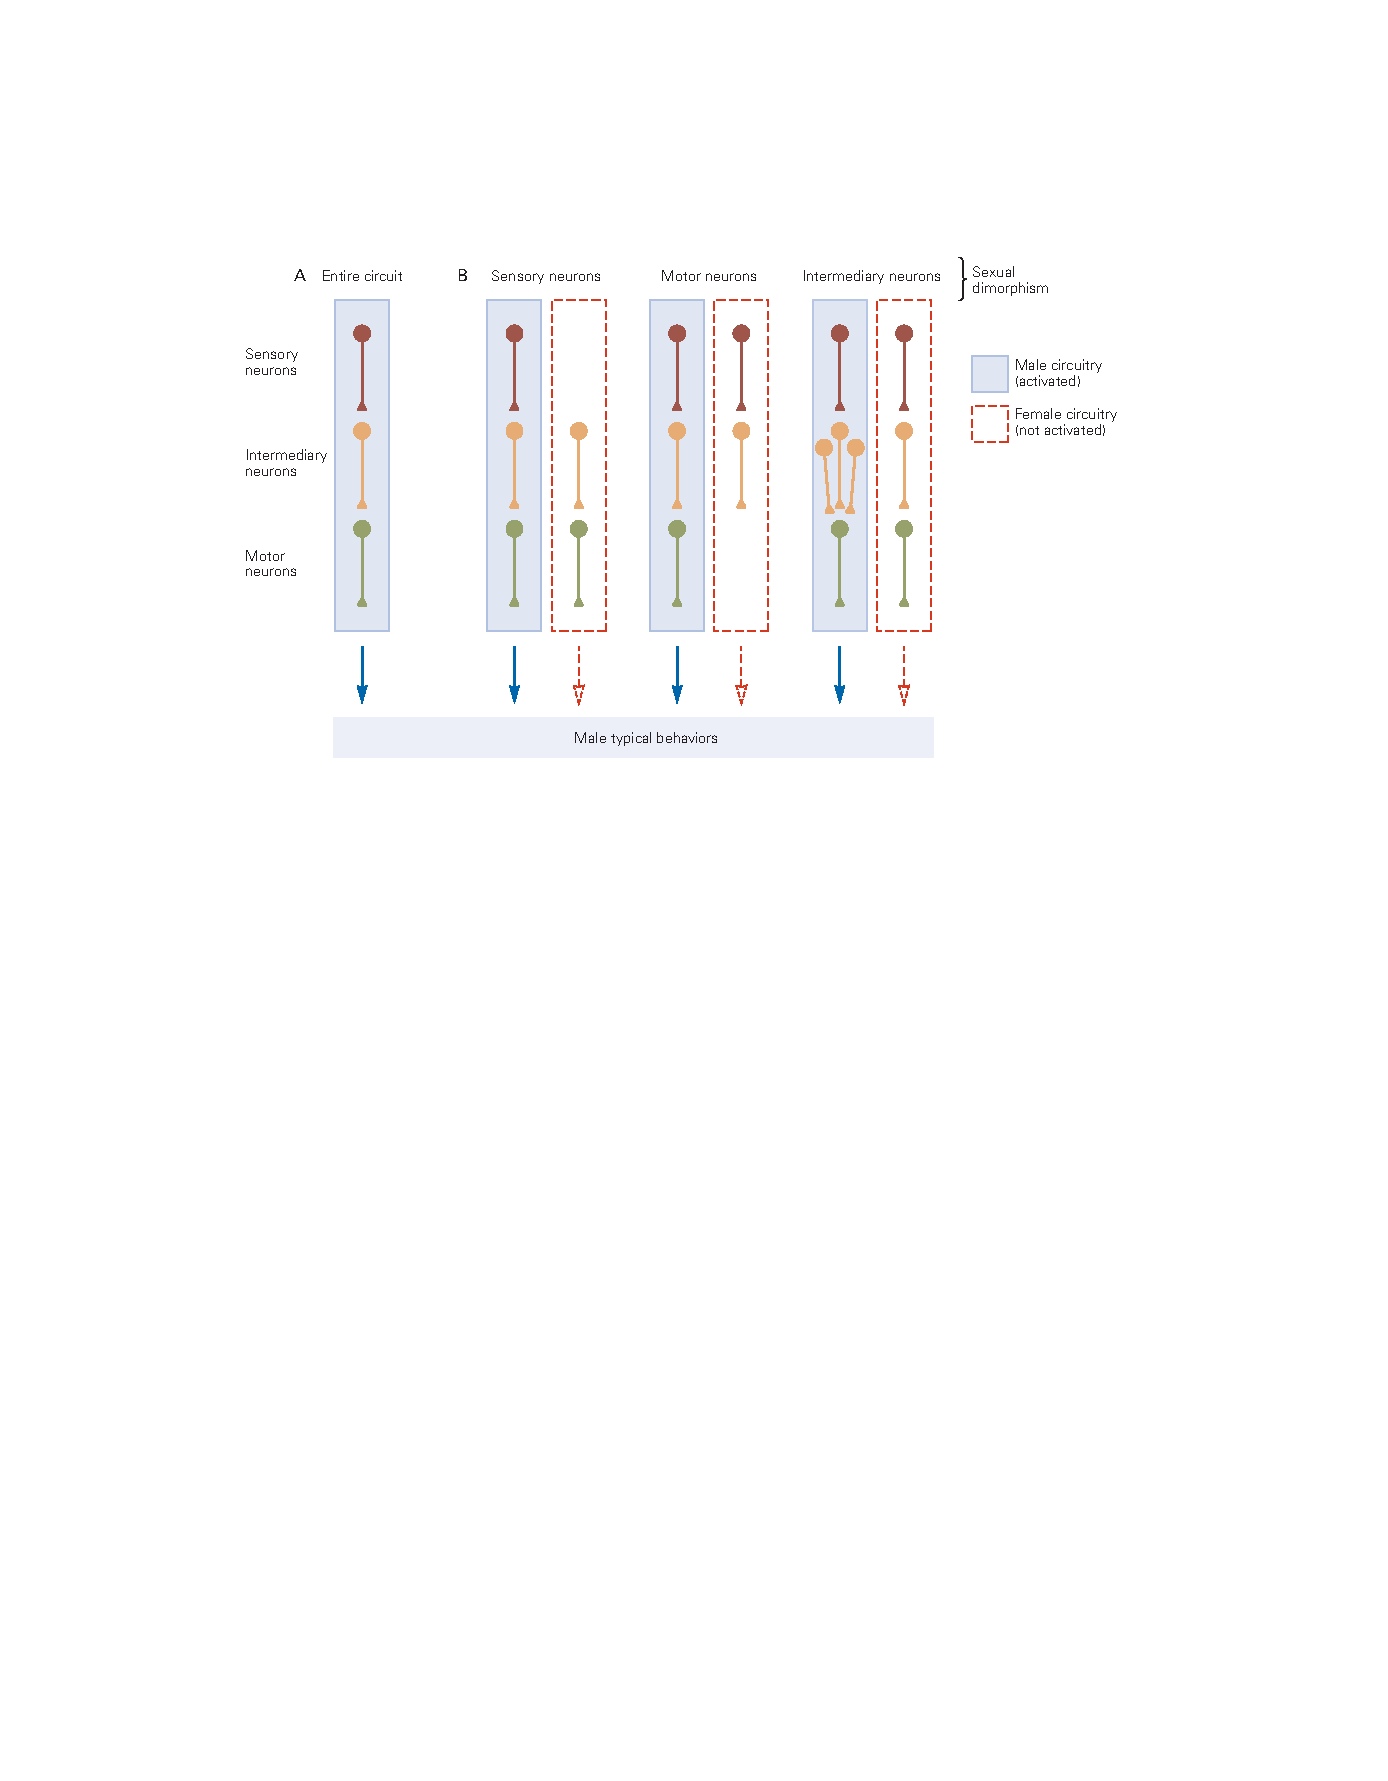
\includegraphics[width=1.0\linewidth]{chap51/fig_51_11}
	\caption{行为性别差异背后的可能回路配置。
		神经回路图可以配置为产生行为的性别差异。
		尽管可以设想一种完全专用于一种或另一种性别的神经回路,但大多数行为在两性之间是共享的,目前的共识是,行为或生理上的性别差异反映了嵌入在其他共享的关键神经元群体中的性别二态性神经回路。
		这种性别二态性已在感觉神经元、运动神经元(如球海绵体神经元脊髓核所讨论的)或介于感觉和运动通路之间的神经元(例如\textit{终纹床核}和视前区的性二态核)水平上发现。}
	\label{fig:51_11}
\end{figure}


雌激素不仅可以在发育过程中发挥作用,而且还可以在成年小鼠中发挥作用,定期重新配置下丘脑神经回路内的突触前连接,确保雌性小鼠仅在排卵和受精时交配。
这些研究描绘了女性大脑中的动态神经回路图:接线图是可塑的,并且对整个发情周期的荷尔蒙变化有反应,这类似于人类的月经周期。
同样,雌激素也对其他大脑区域的树突棘可塑性产生周期相关的影响,尽管在这些情况下的行为后果不太清楚。


发育中的大脑中另一个反复出现的主题是,男性化在组织阶段受雌激素控制。
这种控制对成人生活中的社会行为具有深远而持久的影响。
睾酮(芳香化为雌激素)或雌性新生啮齿动物的雌激素治疗可使大脑男性化。
作为成年人,这些女性不再接受男性的性行为,并且实际上表现出男性典型的社交互动,尽管强度有所降低。
向这些雌性提供睾丸激素,以模仿成年雄性睾丸激素水平,将社会行为的强度提高到雄性典型水平,包括领土侵略(动物为领土或配偶而战的倾向)。
因此,围产期睾酮的激增主要通过芳构化成雌激素来使大脑男性化,而在成年生活中,睾酮和雌激素都有助于表现出典型的男性社会互动(图~\ref{fig:51_12}A)。


\begin{figure}[htbp]
	\centering
	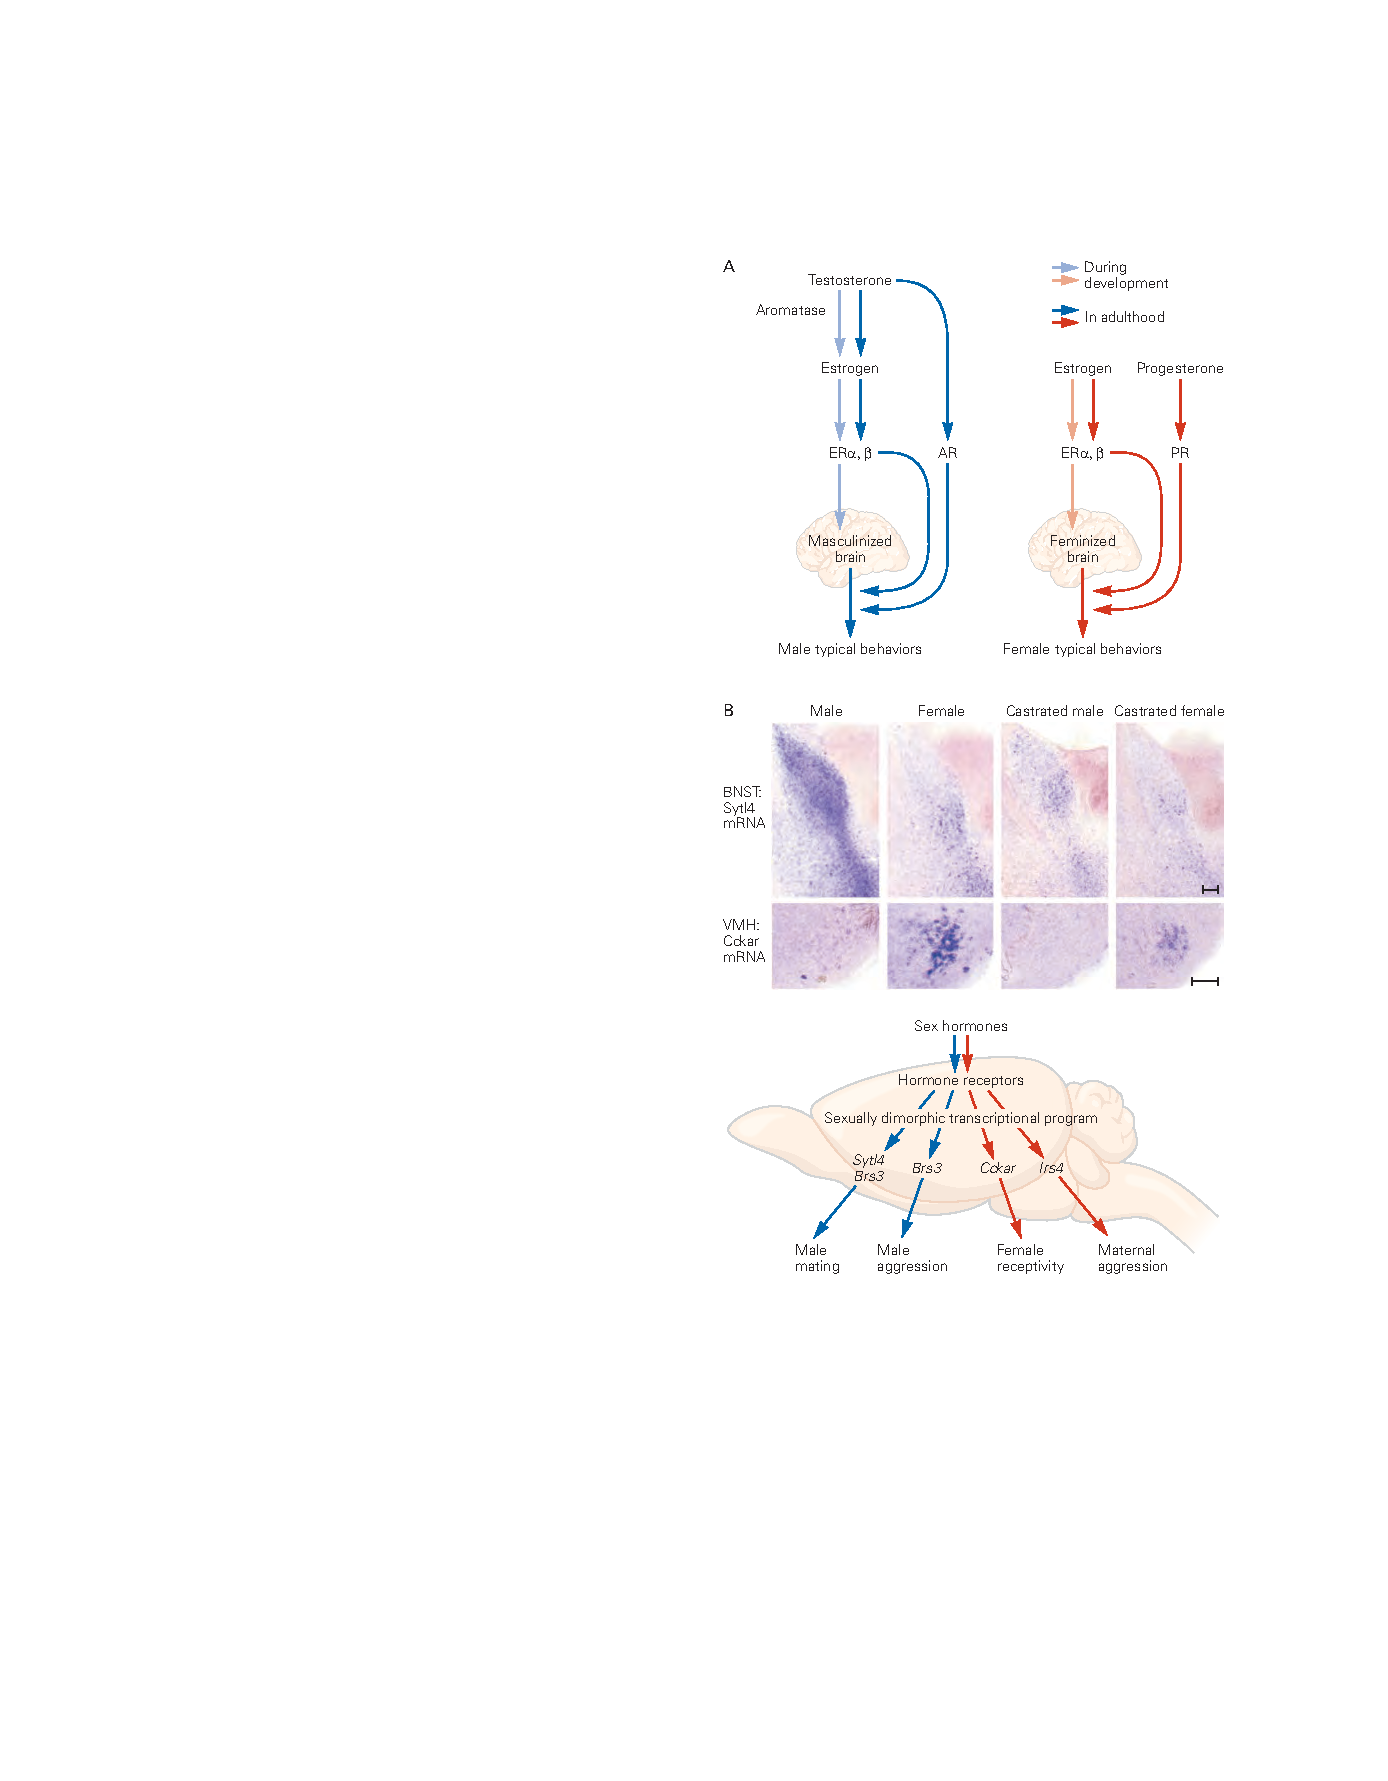
\includegraphics[width=1.0\linewidth]{chap51/fig_51_12}
	\caption{性激素影响神经系统发育和功能的机制。
		\textbf{A.} 神经系统的男性化至少发生在两个不同的步骤中:
		发育组织阶段主要由雌激素信号控制,青春期后激活阶段由雌激素和睾酮信号通过其同源激素受体控制,以调节基因表达。
		\textbf{B.} 组织学图像显示终纹床核\textit{终纹床核}和\textit{腹内侧下丘脑} Cckar 中 Sytl4 \textit{信使核糖核酸}的性二态表达模式 ) 的成年小鼠。
		这些基因的表达在未被操纵的男性和女性中明显不同,并且在成年生活中阉割后通过实验从循环中去除性激素后发生显著变化。
		\textit{终纹床核}和\textit{腹内侧下丘脑}都调节两性的交配和攻击行为。
		下图说明了目前关于性激素如何调节行为的性别差异的思考。
		分子研究已经确定了许多基因,例如 Sytl4 和 Cckar,它们的表达在成人大脑中具有性别二态性,并受性激素控制。
		许多这样的基因,当通过基因工程在老鼠身上进行实验性突变时,可以调节两性异形行为的不同组成部分,但不能调节整个社会互动库。
		换句话说,性激素以模块化的遗传方式控制性二态行为\cite{xu2012modular}。}
	\label{fig:51_12}
\end{figure}


这些发现表明,仅在神经系统中缺乏雄激素受体的雄性小鼠不仅具有雄性生殖器,而且还表现出雄性的社会行为模式,尽管强度有所降低。
事实上,小鼠基因工程研究很好地证实了这一点;
这种突变的雄性小鼠在外观上确实与对照雄性小鼠没有区别,但它们表现出雄性的性行为和攻击行为,但强度有所减弱。
然而,越来越多的证据表明,雌激素对大脑男性化的发育控制在进化过程中发生了变化,因此睾酮可能是包括人类在内的灵长类动物的主要男性化因子。


有限数量的性激素的作用如何调节大量复杂社会互动的表现,例如求爱发声(类似于鸣禽,许多动物,包括老鼠,发声作为它们交配仪式的一部分)、性行为、标记 (许多物种的动物倾向于通过体液中分泌的信息素来占领领地)和侵略性?
如本章前面所述,性激素与同源受体结合以调节靶细胞中的基因表达。
这些类固醇在两种性别大脑中的可用时间、数量和位置不同。
因此,性激素调节基因以性二态模式表达,不同大脑区域也不同。
这些基因沿着男性或女性典型细胞系调节神经回路的分化和成年功能(图~\ref{fig:51_12}B)。


这种性激素调节基因的实验失活表明,个体基因仅影响两性社会互动的一部分,而不会改变男性和女性的整个行为程序。
因此,另一个新兴主题是性激素以模块化方式控制神经回路的分化和功能,不同的性激素调节基因作用于不同的神经元群体,以调节男性或女性典型行为的不同方面。
简而言之,没有单一的神经元群体可以控制典型的性别行为;
相反,不同行为的神经控制分布在多个不同的神经元群体中。


这种对性二态行为的模块化控制非常符合我们的想法,即大多数回路在男性和女性之间共享,并且行为中的性别差异是由关键的神经群体引起的,这些神经群体以典型的男性或女性方式改变回路功能。
表现出性二态性分子或解剖学特征的神经元似乎代表了这些关键的神经元群体。



\section{人脑是两性异形的}

雄性和雌性哺乳动物大脑之间的性别差异是否也存在于人类身上?
如果存在,它们在功能上是否重要?
早期研究表明,男性的一些结构明显更大。
这些包括脊髓中的\textit{奥奴弗罗维奇核},啮齿动物中\textit{球海绵体肌脊髓核}的同系物(图~\ref{fig:51_7});
\textit{终纹床核},与啮齿动物交配行为有关(图~\ref{fig:51_4});
和\textit{下丘脑前间质核}3,与前面讨论的啮齿动物 SDNPOA 相关(图~\ref{fig:51_13})。


\begin{figure}[htbp]
	\centering
	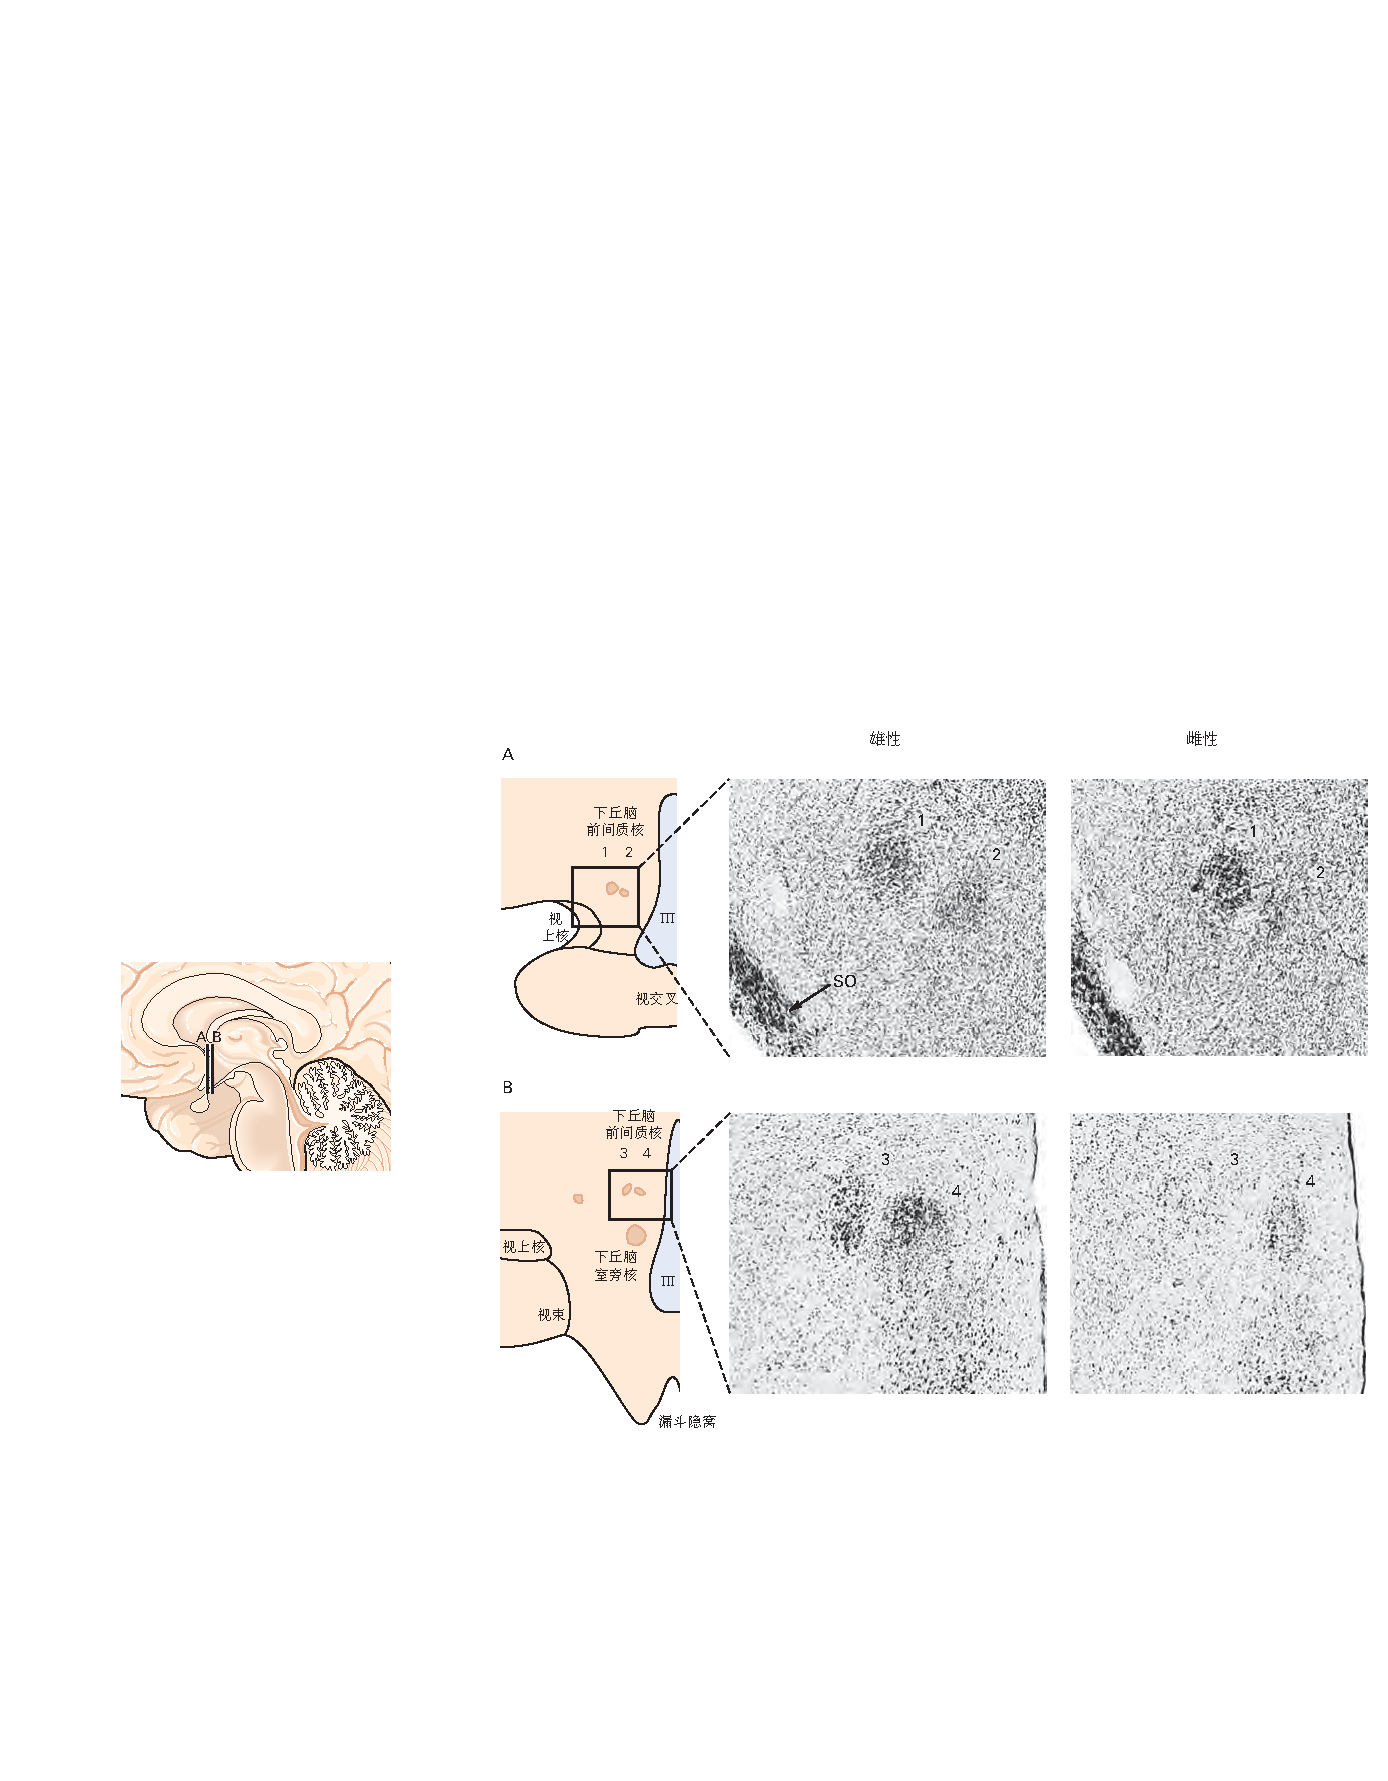
\includegraphics[width=1.0\linewidth]{chap51/fig_51_13}
	\caption{人脑\textit{下丘脑前间质核} 3 的性别二态性。
		人类下丘脑包含四个小的、离散的神经元簇,\textit{下丘脑前间质核} 1 到 \textit{下丘脑前间质核} 4。
		显微照片显示了成年男性和女性大脑中的这些细胞核。
		虽然\textit{下丘脑前间质核}1、\textit{下丘脑前间质核}2 和\textit{下丘脑前间质核}4 在男性和女性中看起来相似,但\textit{下丘脑前间质核}3 在男性中明显更大。\cite{gorski1988hormone} }
	\label{fig:51_13}
\end{figure}


高分辨率\textit{核磁共振成像}和组织学的进步揭示了中枢神经系统中更微妙的结构和分子二态性。
例如,与一群成年男性相比,成年女性的额眶皮层和几个脑回(包括中央前回、额上回和舌回)等结构占据的体积明显更大(图~\ref{fig:51_14})。
此外,与女性相比,男性的额内侧皮层、杏仁核和角回体积更大。
因此,人脑中可能存在许多性别二态性。


\begin{figure}[htbp]
	\centering
	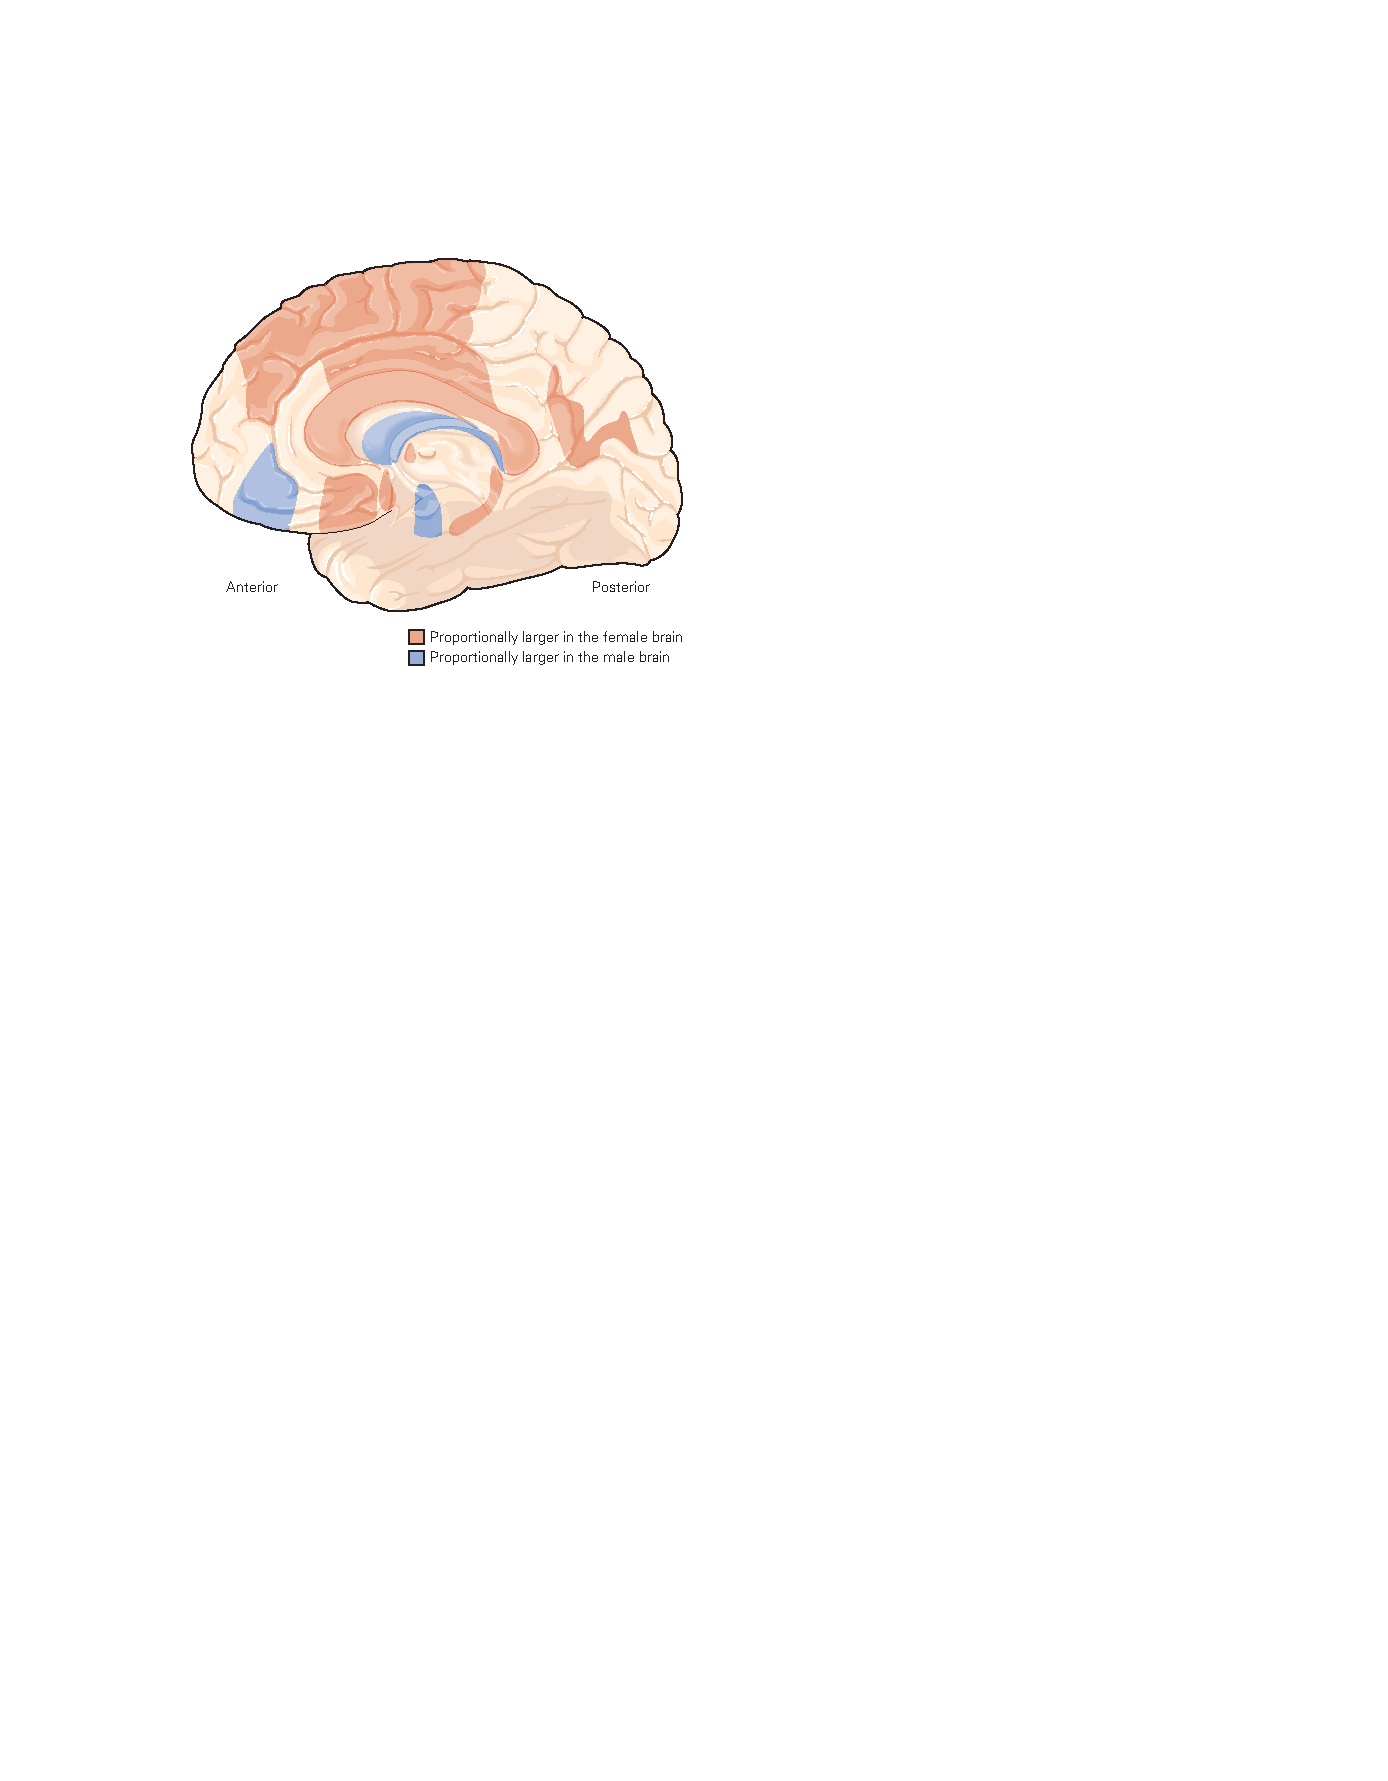
\includegraphics[width=0.63\linewidth]{chap51/fig_51_14}
	\caption{性二态性在成年人脑中很普遍。
		一项磁共振成像研究测量了成年男性和女性许多大脑区域的体积。
		每个区域的体积被归一化为两种性别的大脑大小。
		性别差异在许多区域都很显著,包括几个可能调节认知功能的皮层区域\cite{cahill2006sex}。 }
	\label{fig:51_14}
\end{figure}



\subsection{人类的性别二态性可能源于荷尔蒙作用或经验}

目前尚不清楚这些大脑二态性是如何产生的,以及它们与行为的关系。
它们可能早期因荷尔蒙的组织效应而出现,或后来因经验而出现。
出生前或出生后不久出现的性别差异可能是行为差异的基础,而出生后出现的性别差异可能是二态经历的结果。
在少数情况下,这些问题的答案相当明确。
例如,对啮齿动物负责阴茎勃起和哺乳的神经回路发育的研究很容易转化为人类。


最近的两项观察表明,首先在动物身上研究的经验对行为的持久影响(图~\ref{fig:51_10})也与人类相关。
首先,正如第~\ref{chap:chap49}~章所讨论的,长期在孤儿院中缺乏个人照顾的儿童在各种社会行为方面存在长期缺陷。
即使在被安置在寄养家庭多年后,这些孩子的血清中催产素和加压素的平均水平仍低于亲生父母抚养的孩子。
其次,小时候遭受虐待的人长大后往往成为贫穷的父母。
尸检研究表明,与对照人群中的成年人相比,儿童时期受过虐待的成年人其糖皮质激素受体基因的启动子甲基化程度更高。
虽然这些研究是新的并且需要重复,但它们提供了关于早期父母照顾终生影响的生物学机制的诱人线索。



\subsection{大脑中的双态结构与性别认同和性取向相关}

与绘制人类一些相对简单的两性异形行为的生物学基础的进展相比,对性伴侣偏好和性别认同的差异仍然知之甚少。
在将认知功能的性别差异与大脑结构差异联系起来方面进展甚微,部分原因是认知差异的存在本身仍然是一个有争议的问题;
如果它们存在,它们也很小,代表高度可变的男性和女性人口之间的均值差异。
另一方面,一些证据表明性别认同和性取向的明显差异与大脑中的二态结构有关。


对这个问题的早期洞察来自对具有单基因突变的人的观察,这些突变将解剖性别与性腺和染色体性别分离,例如\textit{雄激素不敏感综合症}、\textit{先天性肾上腺皮质增生症}和 5$\alpha$-还原酶缺乏症(表~\ref{tab:51_1})。
例如,患有\textit{先天性肾上腺皮质增生症}的女孩在胎儿期经历了过量的睾酮;
这种疾病通常在出生时就被诊断出来并得到纠正。
然而,早期接触雄激素与随后性别相关行为的变化相关。
平均而言,患有\textit{先天性肾上腺皮质增生症}的女孩往往有玩具偏好,并且会参与同龄男孩的典型游戏。
在儿童时期接受\textit{先天性肾上腺皮质增生症}治疗的女性中,同性恋和双性恋倾向的发生率也有小幅但显著的增加,并且这些女性中的很大一部分也表达了作为男性生活的愿望,这与性别认同的变化一致。
这些发现表明,类固醇的早期组织效应会影响与染色体和解剖性别无关的性别特异性行为。


在 5$\alpha$-还原酶 II 缺乏症和\textit{雄激素不敏感综合症}中,许多受影响的男性表现出完全女性化的外生殖器,并且在青春期之前被误认为是女性。
此后,他们的历史发生了分歧。
在 5$\alpha$-还原酶 II 缺乏症中,症状是由睾酮加工缺陷引起的,主要局限于发育中的外生殖器。
在青春期,循环睾酮的大量增加使体毛、肌肉组织和最显著的外生殖器变得男性化。
在此阶段,许多但并非所有患者都选择采用男性性别。
相反,在\textit{雄激素不敏感综合症}中,缺陷是由雄激素受体的全身缺陷引起的。
这些患者在青春期月经不来后通常会寻求医疗建议。
与其女性化的外部表型一致,大多数\textit{雄激素不敏感综合症}患者表现出女性的性别认同和对男性的性偏好。
他们选择手术切除睾丸和补充适合女性的荷尔蒙。


是什么导致了不同的结果?
在众多可能性中,一种是 5$\alpha$-还原酶 II 患者在青春期行为的显著变化是由作用于大脑的睾丸激素的影响引起的。
在\textit{雄激素不敏感综合症}患者中,这些影响不会发生,因为大脑中没有雄激素受体。
然而,显然,这种解释并不排除社会和文化教养是决定性别认同和性取向的重要因素。


第二组探索性取向生物学的研究评估了对信息素的反应。
人类对信息素的感知与老鼠的感知截然不同,可能是一种不太重要的感觉。
人类没有功能性\textit{犁鼻器},大多数与小鼠\textit{犁鼻器}信息素接收有关的基因,如 trpc2 和编码\textit{犁鼻器}受体的基因,在人类基因组中不存在或无功能。
就人类确实感知信息素的程度而言,他们似乎使用主要的嗅觉上皮细胞和球。
似乎是人类信息素的化学物质包括有气味的雄激素代谢物\textit{雄二烯酮}和有气味的雌激素代谢物\textit{雌四烯醇}。
\textit{雄二烯酮}在男性汗液中的浓度是女性汗液中的 10 倍,而\textit{雌四烯醇}在孕妇尿液中的浓度高出 10 倍。
这两种化合物都可以产生性唤起:对异性恋女性和\textit{雌四烯醇}对异性恋男性,即使浓度很低以至于没有有意识的嗅觉感知。


由\textit{雄二烯酮}和\textit{雌四烯醇}激活的大脑区域已通过\textit{正电子发射断层成像}成像识别。
当出现\textit{雄二烯酮}时,某些下丘脑核团在异性恋女性而非异性恋男性中被激活,而当出现\textit{雌四烯醇}时,包含核团簇的相邻区域在男性中被激活但在女性中没有(图~\ref{fig:51_15}A)。
在同性恋男性和女性中,下丘脑激活发生逆转:\textit{雄二烯酮}而不是\textit{雌四烯醇}激活同性恋男性的下丘脑中枢,相反,\textit{雌四烯醇}而不是\textit{雄二烯酮}激活女同性恋女性的这些区域。
因此,异性恋和同性恋的大脑似乎以不同的方式处理嗅觉信息。


\begin{figure}[htbp]
	\centering
	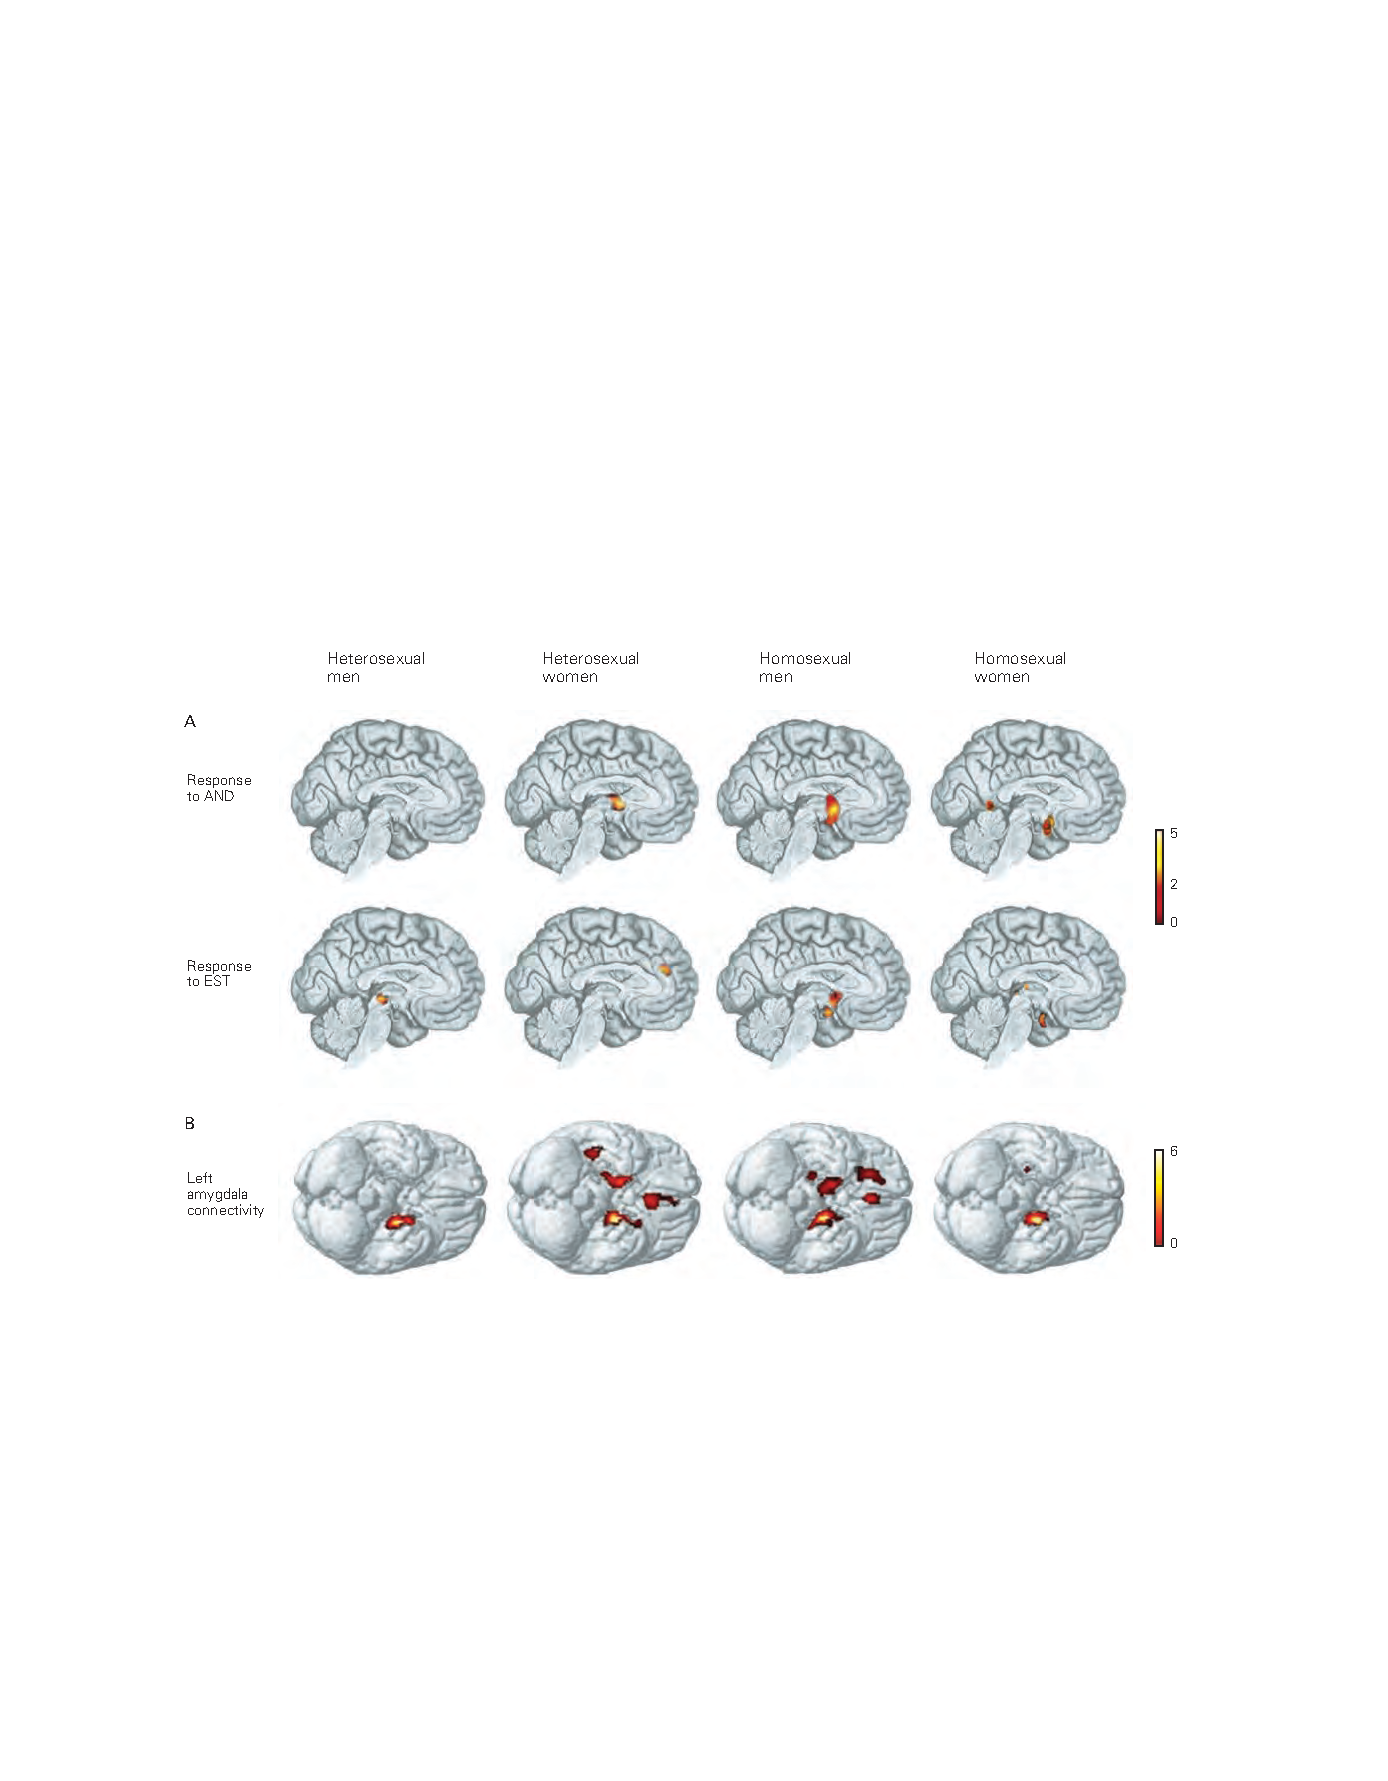
\includegraphics[width=1.0\linewidth]{chap51/fig_51_15}
	\caption{大脑中嗅觉激活的一些性别二态模式与性取向相关。
		\textbf{A.} 与无味空气相比,正电子发射断层扫描成像用于识别受试者\textit{雄二烯酮}或\textit{雌四烯醇}时被激活的大脑区域。
		\textit{雄二烯酮}激活了异性恋女性而非男性大脑中的几个下丘脑中枢,而\textit{雌四烯醇}激活了异性恋男性而非女性大脑中的几个下丘脑中枢。
		同性恋男性下丘脑的激活模式与异性恋女性对\textit{雄二烯酮}的反应相似,而异性恋男性和同性恋女性对\textit{雌四烯醇}的反应也存在类似的激活模式。
		右侧的颜色校准显示了假定的神经活动水平。
		由于选择了相同的大脑部分进行比较,因此该图并未说明每种情况下的最大激活\cite{berglund2006brain}。
		\textbf{B.} 在呼吸无味空气时对异性恋和同性恋受试者进行扫描,并使用协方差测量来估计区域之间的连通性。
		在异性恋女性和同性恋男性中,左侧杏仁核与右侧杏仁核紧密相连,而在异性恋男性和同性恋女性中,连接性仅局限于局部\cite{savic2008pet}。}
	\label{fig:51_15}
\end{figure}


同性恋大脑中的性二态结构是否与解剖性别或性取向相关?
影像学研究支持这样的观点,即同性恋男性的大脑类似于异性恋女性的大脑,而同性恋女性的大脑类似于异性恋男性的大脑(图~\ref{fig:51_15}B)。
此外,与男性相比,男变女变性者的性二态性\textit{终纹床核}体积较小,而女变性者与女性相比似乎具有更大的\textit{终纹床核}(图~\ref{fig:51_16})。
然而,尚不清楚这些个体的结构二态性是性别认同或性取向的结果还是原因。


\begin{figure}[htbp]
	\centering
	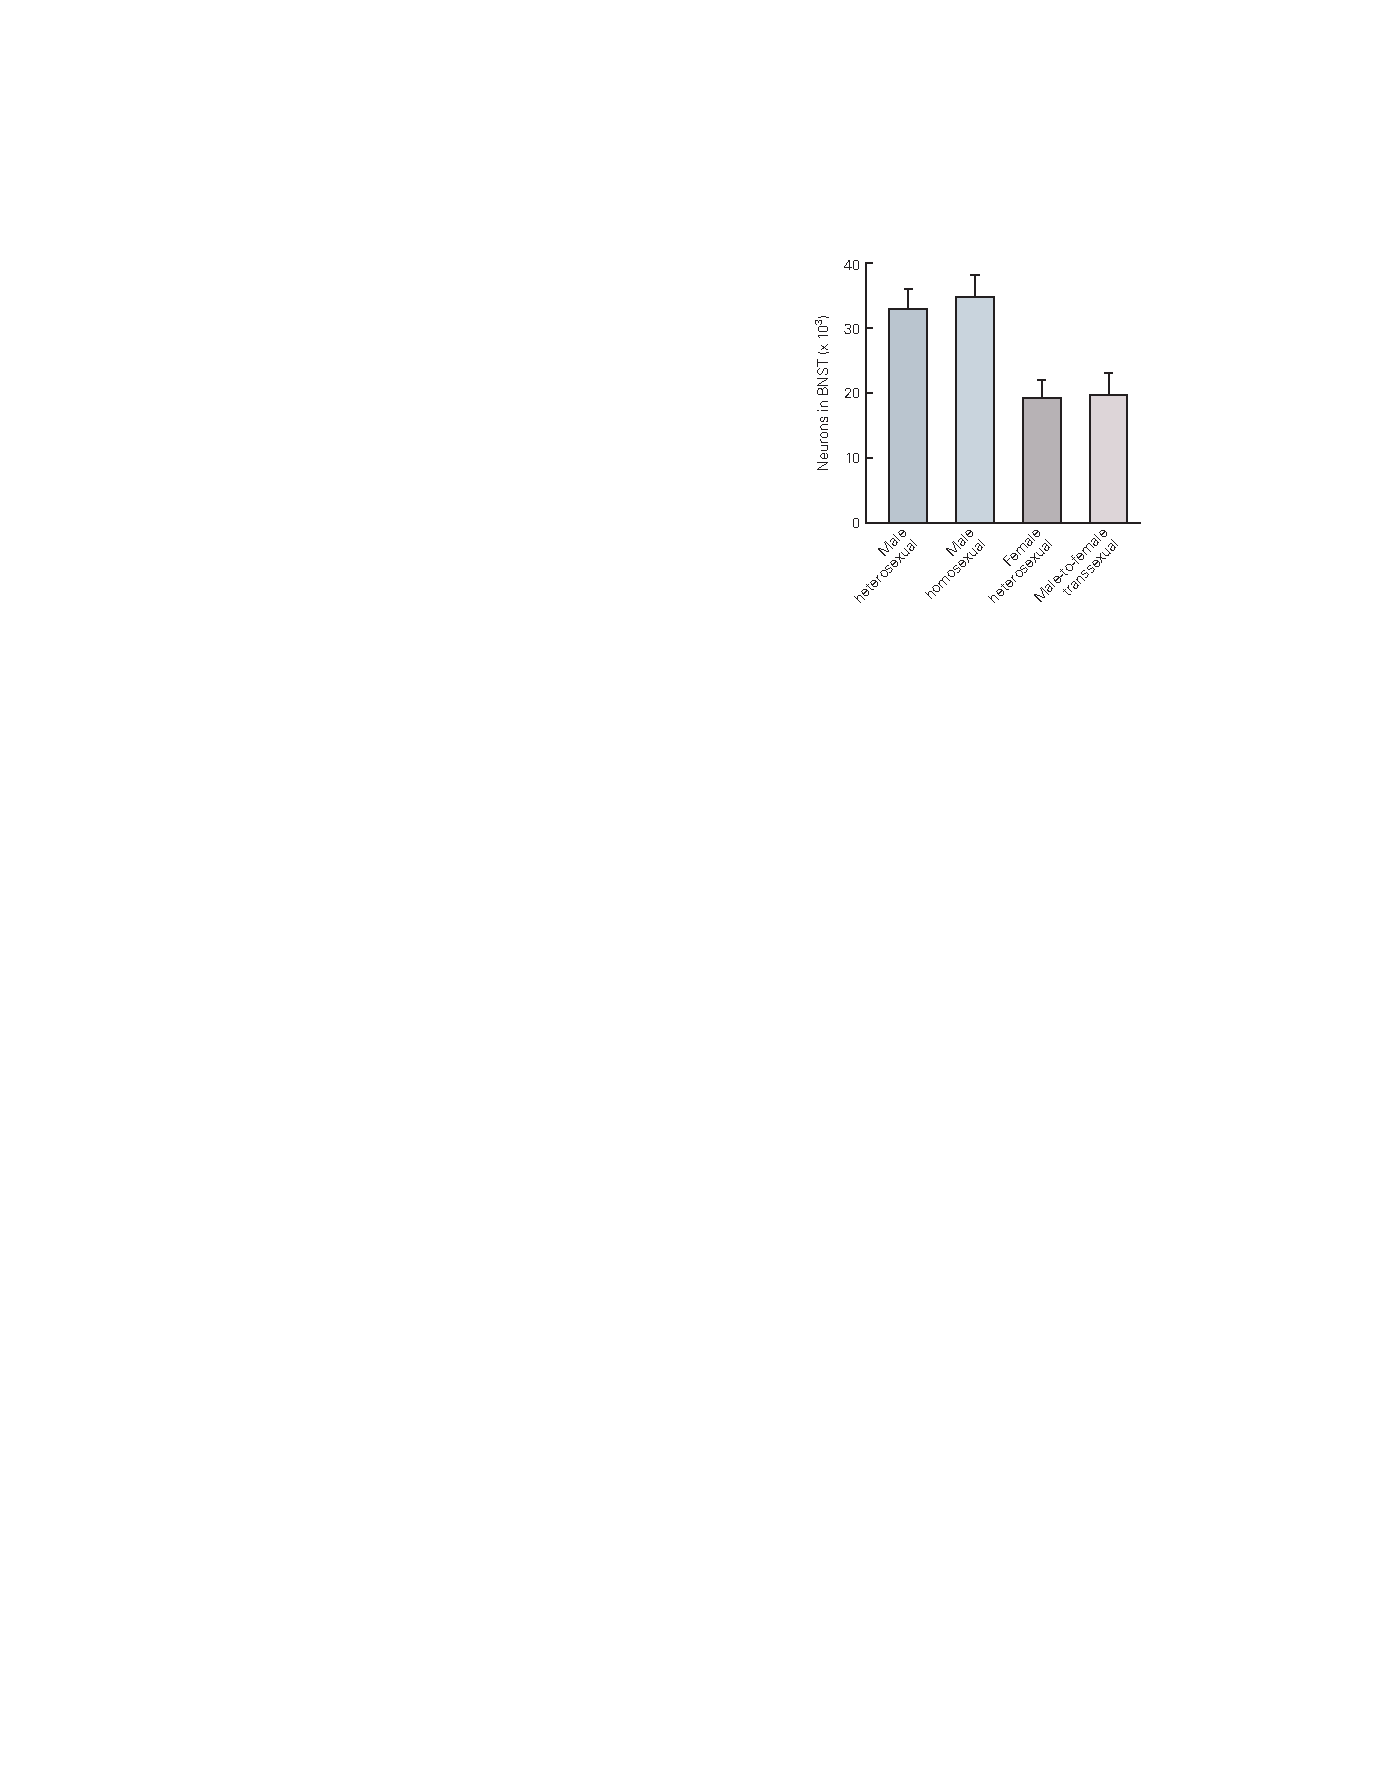
\includegraphics[width=0.51\linewidth]{chap51/fig_51_16}
	\caption{人类\textit{终纹床核}的性别二态性。
		无论男性性取向如何,与女性相比,男性的细胞核具有更多的神经元。
		与女性相似,男变女的变性人的神经元数量少于男性。
		在一个可用于尸检分析的女性变性男性大脑中(未显示在条形图中),神经元的数量完全在男性的正常范围内\cite{kruijver2000male}。}
	\label{fig:51_16}
\end{figure}


人类\textit{终纹床核}的雄性小鼠对应物在识别其他小鼠的性别和指导随后的社会互动方面起着关键作用,例如与雄性的攻击和与雌性的交配。
因此,人类大脑中与性别认同相关的区域在啮齿动物的性别识别中起着重要作用。
与前面讨论的小鼠\textit{终纹床核}的性二态性情况一样,荷尔蒙的影响也被认为是人类\textit{终纹床核}的二态性的基础。


如果产前影响确实导致性别与性别的分离,那么这些影响是遗传的吗?
除了前面描述的罕见综合症外,寻找性取向或性别认同的遗传基础的尝试并未取得成果。
声称的遗传贡献很小,并且尚未复制与特定基因组位点关联的声明。
因此,虽然目前的证据支持早期甚至产前因素在这些过程中的某些贡献,但它们的原因和相对重要性仍然未知。


\section{要点}

1. 在人类和许多其他哺乳动物中,性别决定途径指导双能性腺分化为雄性睾丸和雌性卵巢。
Y 染色体上的 Y 染色体性别决定区基因指导性腺形成睾丸,而 Y 染色体性别决定区基因的缺失使性腺分化为卵巢。


2. 性腺产生的性类固醇激素(睾丸激素和雌激素以及卵巢产生的黄体酮)驱动神经系统和身体其他部分的性别分化。


3. 性激素在发育的关键窗口早期发挥作用,以不可逆的方式组织神经基质以进行性二态性行为,而在成年生活中,这些激素以敏锐和可逆的方式起作用,以激活典型的性别生理和行为反应。


4. 在关键窗口期间,睾丸会产生短暂的睾丸激素激增,使发育中的双潜能神经系统男性化。
相比之下,卵巢在此期间处于静止状态,并且认为性激素的缺乏使神经系统在此期间能够沿着女性典型途径分化。


5. 睾酮使神经系统男性化的许多作用发生在其在作用部位局部转化为雌激素之后。
有证据表明,在人类和其他灵长类动物中,睾酮还直接通过其同源激素受体发挥作用,影响行为神经基质的男性化。


6. 性激素通过利用在其他发育事件中广泛使用的细胞过程,例如细胞凋亡、神经突延伸和突触形成,来控制神经通路的性分化。


7. 性激素与调节基因表达的同源激素受体结合。
这些基因反过来调节导致神经元数量、连接性和生理学性别差异的细胞过程。


8. 在过去的几十年里,脊椎动物的大脑中发现了许多根据形态学和其他标准具有性别二态性的神经元群。
功能研究表明,这些区域影响一些但不是全部的两性异形行为。


9. 最近的分子研究发现了许多性激素调节基因,它们的表达模式是两性异形的。
这些基因以及它们所表达的神经元以模块化方式调节两性异态的社会行为。
换句话说,单个基因和表达它们的神经元群体调节一种或几种性二态行为,因此对这些行为的控制分布在许多不同的神经元群中。


10. 这种性别二态的神经元群体可能嵌入在两性的神经回路中,并且它们被认为可以引导男性或女性典型模式的行为。


11. 感官刺激和过去的经验都深刻地调节了两性异形行为的表现。
在某些情况下,过去经验的影响可以延伸到动物的整个生命周期。


12. 信息素指导啮齿动物选择性伴侣。
影像学研究的证据表明,男性和女性也可能对男性和女性信息素表现出两性神经反应,并且这些反应可能与性取向相一致;
然而,在这些情况下,尚不清楚神经反应是否是基于过去经验的习得反应。


13. 男女大脑之间存在许多性别差异,在某些情况下,这些性别差异与成年生活中的性别一致,而不是出生时指定的性别。
在这些情况下,尚不清楚性别差异是因果反映了性别认同还是性别认同的结果。
这些问题目前很难解决。



